\section{Physical Simulation Studies}
%% TODO - channel level heatmap for neutrino event

We now discuss the methodologies of the physical simulations used as input to the digital tile simulation described in the previous section.

\subsection{Radiogenic Backgrounds as a Calibration Source}

In this section we comment on the ability to, but do not perform, the auto-calibration of the reset loss per charge.
The full charge calibration procedure is beyond the scope of the work presented here, due to intracies that depend on the final implementation of the reset circuit as well as the replenishment circuit of the final Q-Pix ASIC.
Since this ASIC does not yet exist, the true verification of this methodology is not yet possible.
Nevertheless, we desribe the relevant portions to the problem here, since the charge calibration along with the frequnecy calibration and timestamp measurements determine Q-Pix's z-position reconstruction.

The main idea behind the auto-calibration of charge at the pixel level relies on using the known (and near constant) input current from the radiogenic backgrounds (mostly $^{39}$Ar) in the detetor. 
If a perfectly known and constant input current ($I_{o}$) source was input to a pixel it would produce a resets separated by a constant time ($\tau_{rtd}$).
It would be a straight foward matter to calculate the charge per reset: $Q_{o} = I_{o}*\tau_{rtd}$.

Then, to analyze the ability for an auto-calibration procedure for Q-Pix it is important to analyze and understand the long-running charge accumulation (resets) from backgrounds present in the LAr.
We use the following list of radiogenic sources of 10 distinct runs of 1000 seconds each.
Further details on radiogenic backgrounds in LAr can be found at~\citep{DUNE-FD_TDRv4:Abi_2020, ar39_backgrounds, phd_backgrounds}

\begin{table}
\begin{centering}
\begin{tabular}{|p{15mm} p{15mm} p{20mm} p{20mm} p{20mm} p{35mm} |}
 \hline
 Isotope & Rate [Bq/kg] & Region & Region Mass [kg] & Rate [Bq] & Number of Decays (per 10 s window) \\ [0.5ex]
 \hline\hline
  $^{210}$Po & 0.2 & PD [Bq/$m^2$] & 2.46856 & 0.493712 & 5 \\
  $^{60}$Co & 0.0455 & CPA & 90 & 4.095 & 41 \\
  $^{40}$K & 0.49 & APA & 258 & 1,264.2 & 12,642 \\
  $^{39}$Ar & 1.010 & bulk LAr & ~70,000 & 70,700 & 707,000 \\
  $^{42}$Ar & 0.000092 & bulk LAr & ~70,000 & 6.44 & 64 \\
  $^{42}$K  & 0.000092 & bulk LAr & ~70,000 & 6.44 & 64 \\
  $^{222}$Rn & 0.04 & bulk LAr & ~70,000 & 2800 & 28,000 \\
  $^{214}$Pb & 0.01 & bulk LAr & ~70,000 & 700 & 7,000 \\
  $^{214}$Bi & 0.01 & bulk LAr & ~70,000 & 700 & 7,000 \\
  $^{85}$Kr & 0.115 & bulk LAr & ~70,000 & 8050 & 80,500 \\
 \hline
\end{tabular}
\caption{The radiogenic background distribution is the same as that found in previous work~\citep{qpix:shion}.
For each 1000 ssecond analysis the pre-rounded values are scaled up by a factor of 100 to achieve the correct normalization of events for each isotope.
A key difference between the backgrounds is the origin or source of each background.
Of special note is $^{40}$K whose source location is the APA beams, and whose resets can be distinctly seen in Figure~\ref{fig:background_simulation} as the slightly more active (yellow) region of the APA.
Due to this source alone, it is likely that precise auto-calibration for charges will likely have to account for the pixel location within the APA.
}
\end{centering}
\end{table}
~\label{table:radiogenic_backgrounds}

The well-known C++ based Geant4~\citep{geant4:AGOSTINELLI2003250} simulation toolkit is used to simulate particle decay and ionizing particle interactions within the LAr volume.
We use the energy deposited along the track from each ionizing particle with the W-value for liquid argon (23.6 eV) to determine the number of electrons deposited in the LAr.
The resulting number of electrons are then unifromly deposited over the individual track.
Then we calculate the probability of recombination for each electron following the "modified box" model~\citep{2013JInst...8P8005A}.

The time and location of drift for each electron is calculated with an applied transverse and longitudinal diffusion with values taken from Table~\ref{tab:lar_prop}.
The simulations for all particle interactions are run individually with a uniform random sampling of the initial decay time interval within the 1000 second window.
All of the hits are then sorted by increasing time, so that the first hits read are the hits which occur the earliest.
Sorting the hits by time before accumulating charge ensures that the resets happen at the correct time.

This simulation procudes $\mathcal{O}(10^{11})$ hit interactions which produce $\mathcal{O}(10^{14})$ electrons, which in turn produces $\mathcal{O}(10^{9})$ resets.
To reduce the memory utilization of the simulation the electrons are accumulated on a hit-by-hit bases and are subdivided into a pre-determined 4$\times$4 cross-sectional area of the detector.
Each cross-sectional area defines a pixel.
The dimension of the LArTPC volume is 2.3~$\unit{m}$ $\times$ 6.0~$\unit{m}$ which divides into 575 pixels in the x-direction and 1500 pixels in the y-direction.
There are then a total of 862,500 pixels, which store location and reset information.

As an example, the total resets from 1000 seconds of the simulation are shown in Figure~\ref{fig:background_simulation}.
The most active pixel receives $\approx 220$ resets during this simulation time.
The bins for the histogram are at the pixel level, and represent the 4$\times$4$~\unit{mm^{2}}$ of each pixel.

\begin{figure}[]
\centering
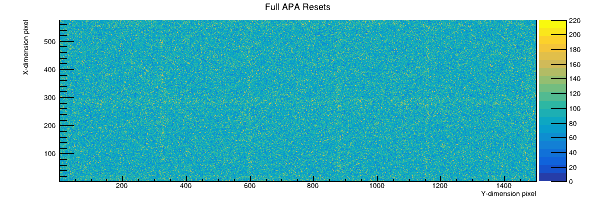
\includegraphics[width=\textwidth]{images/fullApaResets.png}
\caption{Full 1000 second of radiogenic background source simulation input into all pixels within the APA.
A close examination of the resets can reveal the additional resets from the backgrounds which are location dependent.
The majority of the uneven distribution of resets occur at the location of the APA bars due to the $^{40}$K isotope.
}
\end{figure}~\label{fig:background_simulation}

Additional information is tracked for each reset to identify the contribution of each radiogenic background for each reset.
A reset occurs when 6250 $e^{-}$ have accumulated on a pixel.
The time recorded for the reset is the same as the time the simulation calculates the last of the required 6250 electrons to arrive at the designated pixel region.
This optimization was added to the existing simulation framework to separate the unknown analog contribution to the timing uncertainty from the physical simulation.

In practice, the analog front-end reset circuit obviously takes time to respond to added charge and to issue a replenishment and reset commands.
There will always be some delay between the final electron's arrival, the time of the analog reset, the replenishment circuit, and the time recorded on the digital back-end.
However, for the purposes of this analysis, we assume that this reset and replenishment circuit activity can happen more quickly than the average local oscillator of the digital back-end. 
Therefore this analysis assumes the best timing measurement based on the digital back-end.
The time measurement is then limited only by the clock frequency of each local oscillator.
Finally, we comment that this optimization of the timing of the analog front-end affects only the time values, and by extension, the reconstruction of the particle tracks.
It does not affect the total amount of charge, and therefore the total number of resets recorded by each pixel.

Any combination of the backgrounds can contribute some or all of the electrons required to produce a reset.
The contribution of the total electrons for each of the radiogenic sources are shown in Figure~\ref{fig:compare_electron_contribution}.
We refer to the contribution of the number of the electrons to the reset as the "weight" of the reset.

\begin{figure}[]
\centering
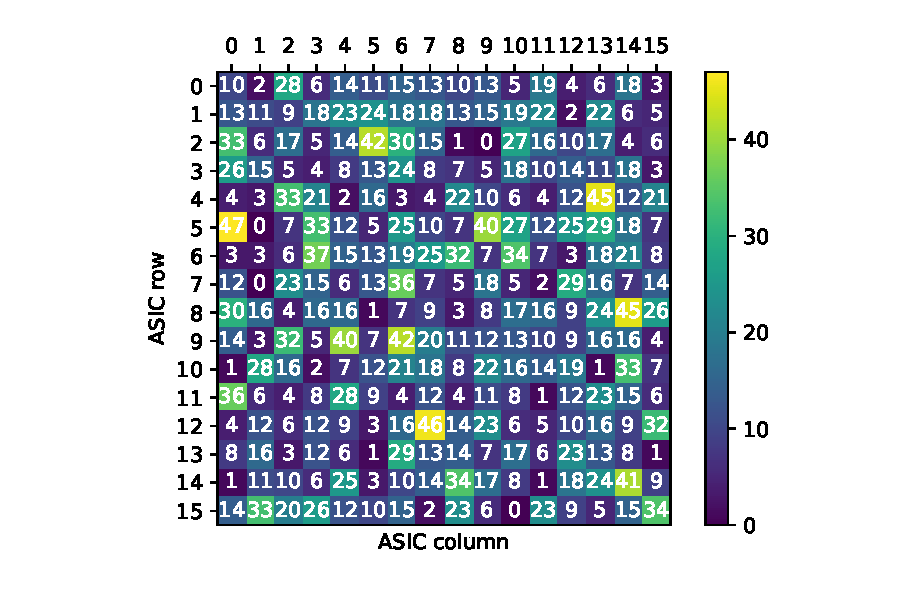
\includegraphics[width=\textwidth]{images/localHitsRadiogenic.pdf}
\caption{Baseline noise input for the digital simulation from all radiogenic sources and background leakage current. 
This figure shows the total resets in the 10 second window for the 16$\times$16 tile.
The other tile size configurations (4$\times$4, 8$\times$8, 10$\times$14) also use these reset data for background noise.
All tiles start with the top left node as their origin node.
}
\end{figure}~\label{fig:reference_input_noise}

%% example RTD for a 16x16 tile
\begin{figure}[]
\centering
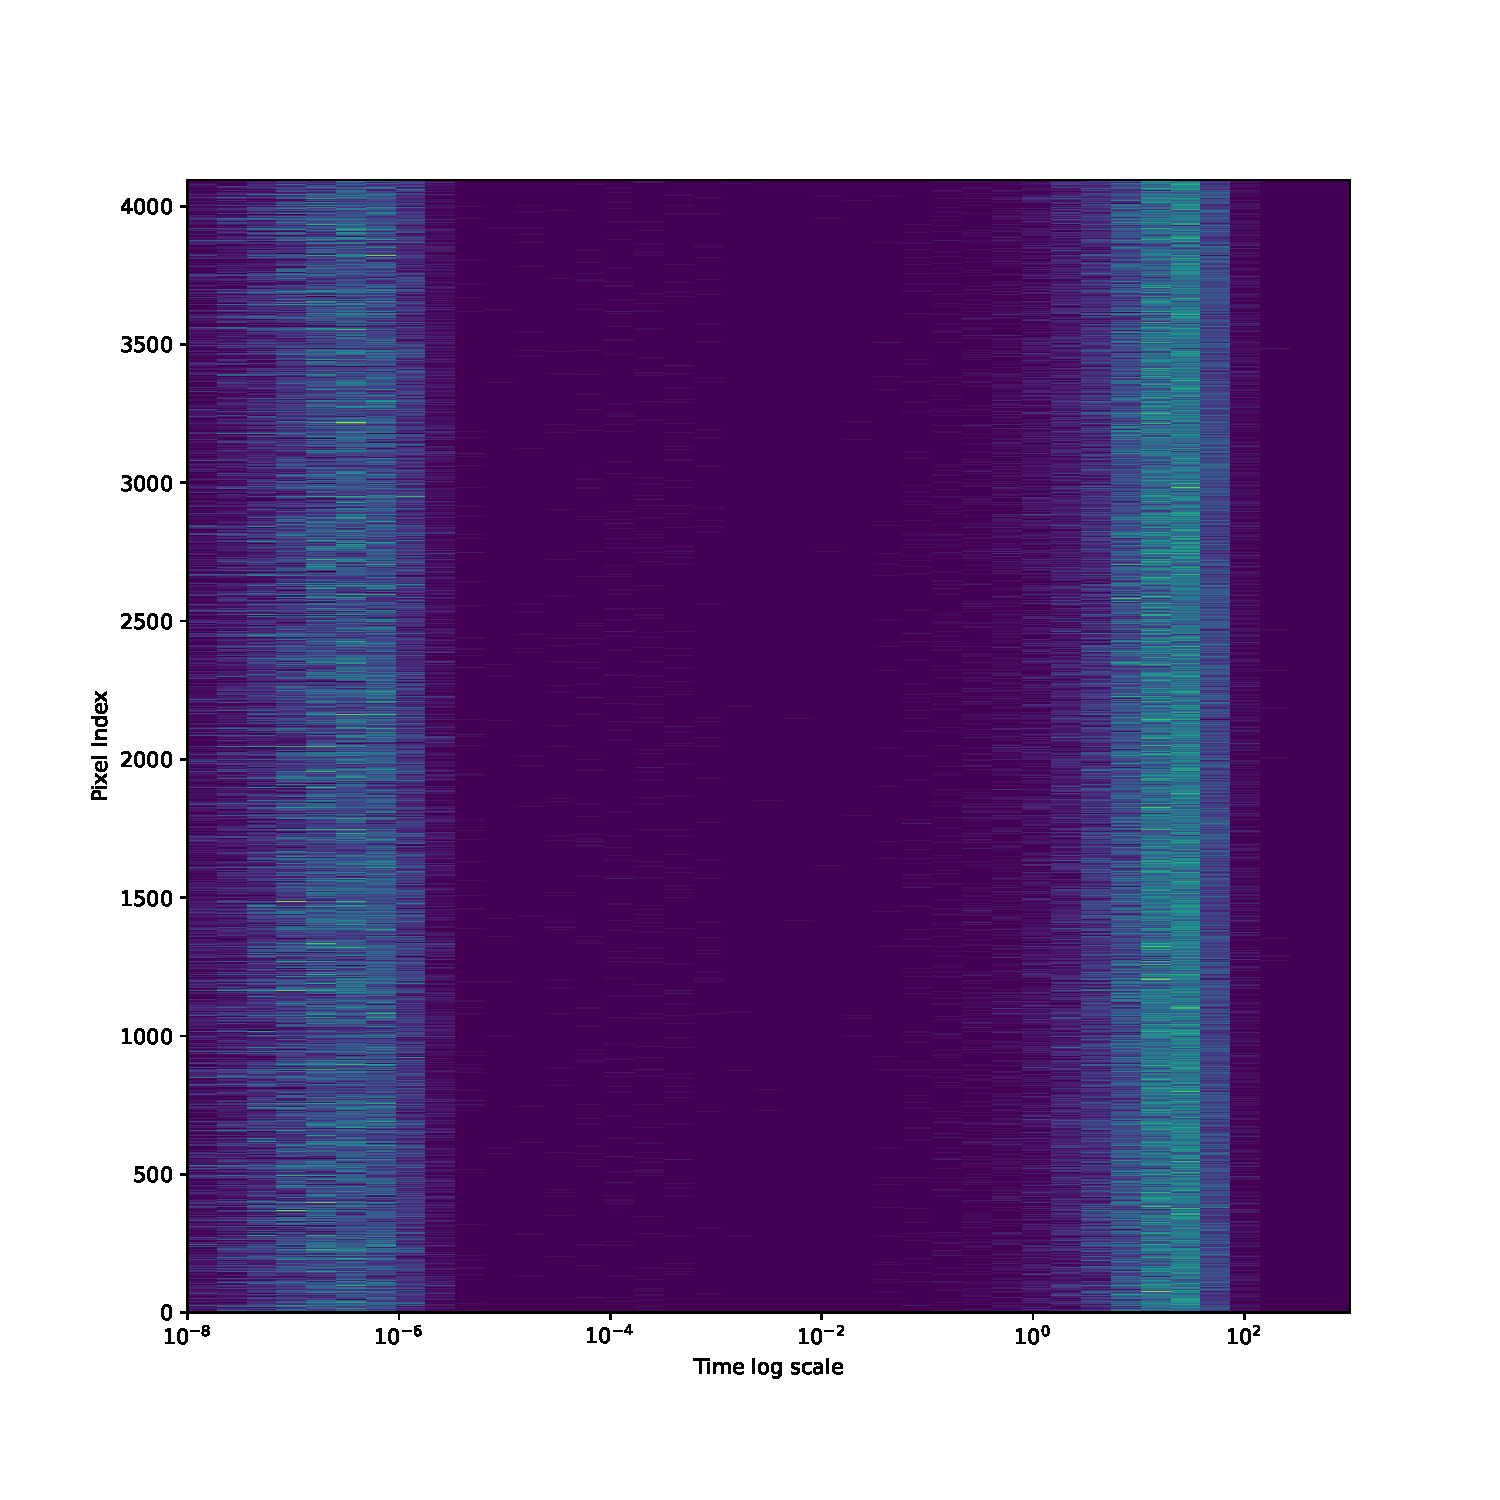
\includegraphics[width=\textwidth]{images/radiogenicRTDtimescale.pdf}
\caption{All 4096 pixels in the 16$\times$16 tile for 1000 seconds of radiogenic data. 
The y-axis represents a different pixel, and the x-axis is a log-scale time axis with even bin widths.
There are to clusters of resets for different time intervals.
The first large cluster of resets occurs at $\approx 10^{-7}$ seconds and is due to a single radiogenic decay event causing additional resets.
The second large cluster of resets occurs at $\approx$ 10 seconds.
This second cluster of resets is caused from the first reset of a new radiogenic decay event.
The ability to perform a charge calibration per pixel may depend on accurately resolving the mean for this "long period" RTD.
 }
\end{figure}~\label{fig:radiogenic_rtd_timescales}

%% time bin of 16x16 tile resets
\begin{figure}[]
\centering
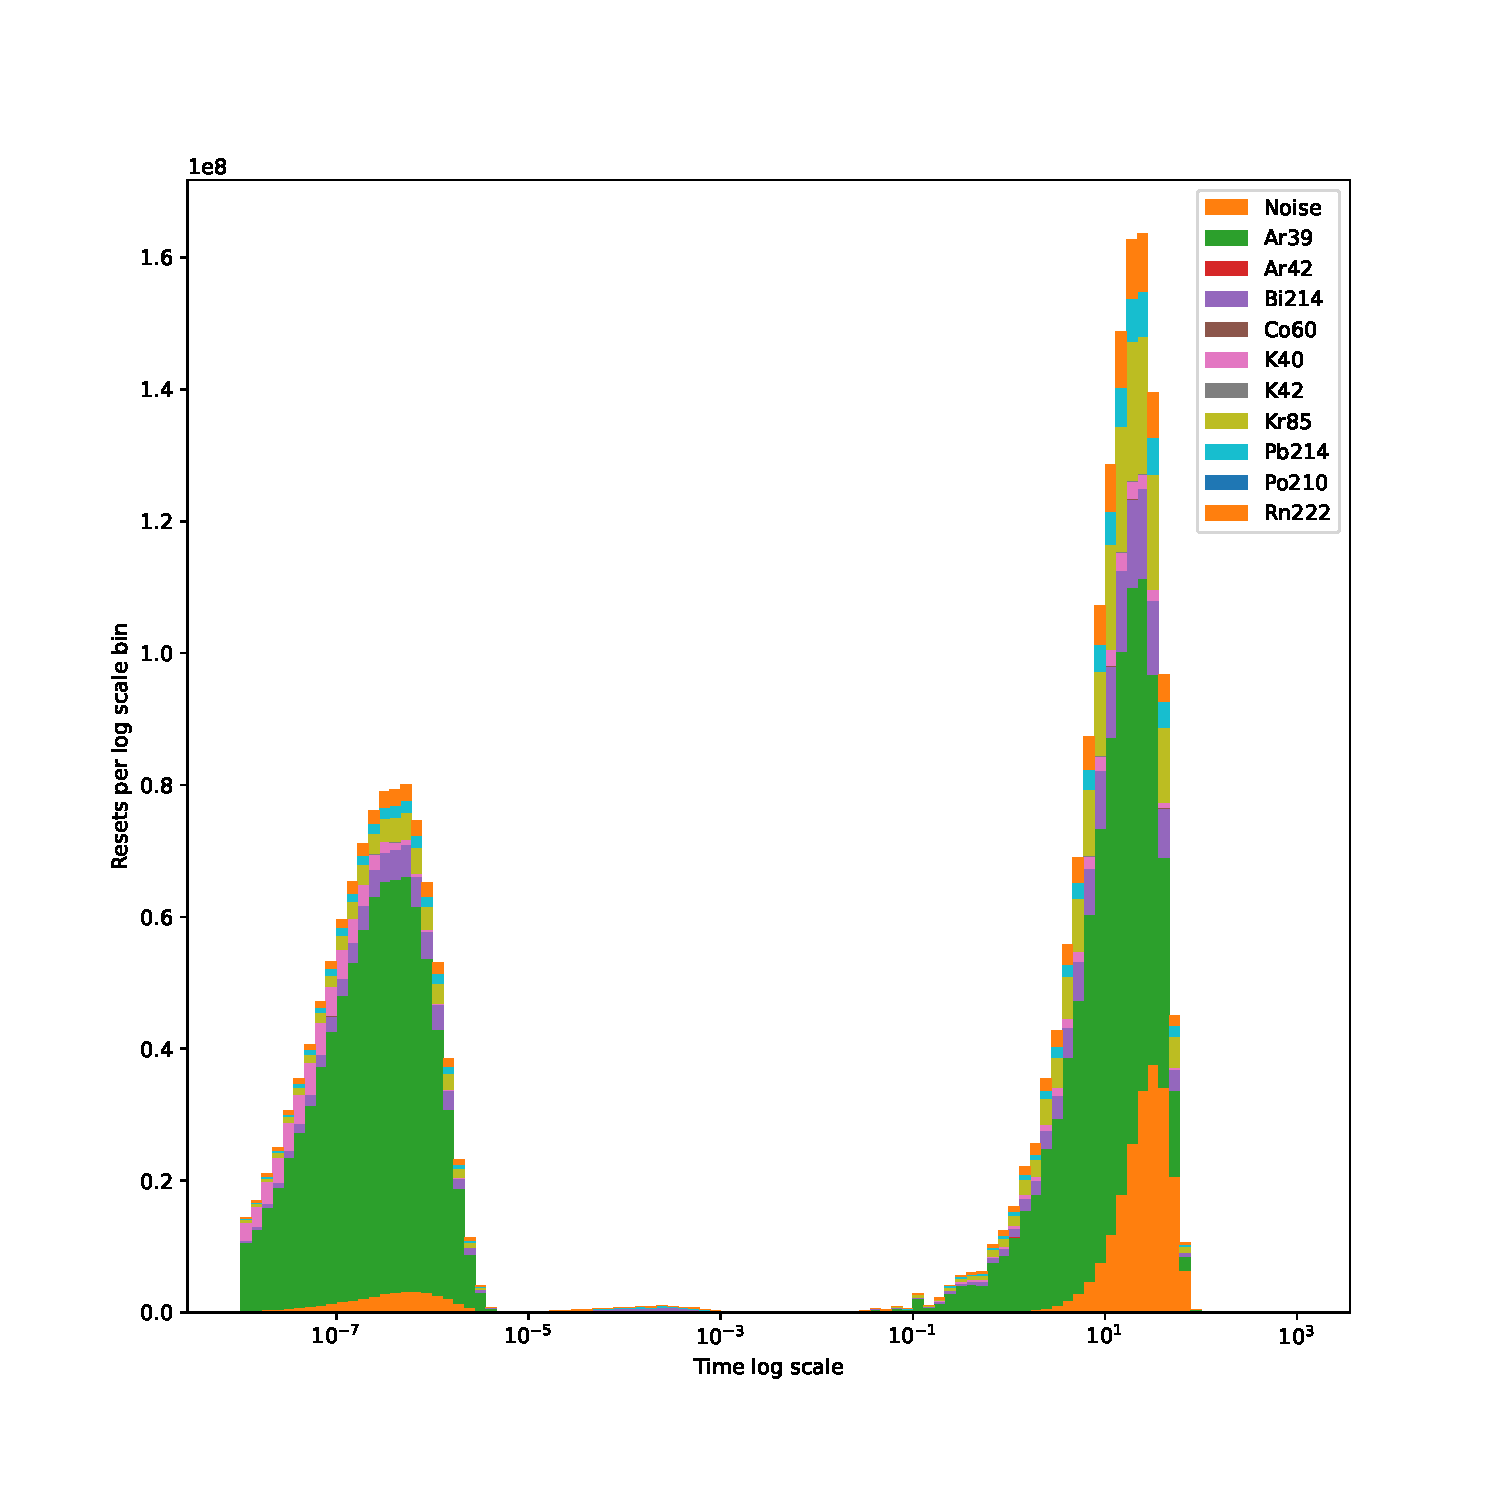
\includegraphics[width=\textwidth]{images/radiogenicRTDtimescale_stack_1d_noise.pdf}
\caption{All 4096 pixels in the 16$\times$16 array for 1000 seconds of radiogenic data. 
These data are the same as those shown in Figure~\ref{fig:radiogenic_rtd_timescales}, where all pixel RTDs are binned together.
There are two clusters of resets on two different time scales.
The first cluster of resets near at $\tau_{rtd} \simeq \mathcal{O}(10^{-7})$ is due to events which produce more than one reset.
The second cluster of resets near at $\tau_{rtd} \simeq \mathcal{O}(10^{1})$ are from a "waiting" period where there is no charge buildup from decays and only background noise.
The dominant source of electrons on each pixel is from the $^{39}$Ar, with a non-zero contribution from leakage.
The leakage current value used in this simulation is 10~\unit{aA}.
}
\end{figure}~\label{fig:radiogenic_rtd_timescales_comparing_no_noise}

The ability to perform a charge auto-calibration using radiogenic events depends on the background to provide a reliable average input current source.
We use only the data presented in Figure~\ref{fig:radiogenic_rtd_timescales} and calculate the mean time between resets for all pixels.
For this simple calculation, we simply take the total number of pixels (4096) and divide by the total number of recorded resets (411152) and obtain and average RTD of 9.96 seconds.

A very rough expectation of background current is $I_o \approx$ 100~\unit{aA}.
We can then use the following equation to calculate:
$$
I_{o} = \frac{Q_{o}}{\tau_{rtd}}
$$

solving for $Q_{o}$ with $\tau_{rtd} = 9.96$ and $I_{o} \approx 100$~\unit{aA}, we obtain:
$$
Q_{o} \approx 100*10^{-18} * 9.96 / 1.6*10^{-19} \approx 6225
$$

More sophisticated analysis will be needed for pixel level charge calibration.
The contrived derivation above assumes equal capacitance and charge replenishment on all pixels, which in practice is not necessarily true.
Furthermore, additional tests can likely be done for each pixel by comparing the peak of the distributions as shown in Figure~\ref{fig:radiogenic_rtd_timescales_comparing_no_noise}.
Such an analysis is not appropriate yet since it is not yet known what the leakage current will be in the Q-Pix ASIC.
As shown in both Figure~\ref{fig:radiogenic_rtd_timescales_comparing_no_noise} and Figure~\ref{fig:compare_electron_contribution}, the contribution from noise is not negligable.
Therefore, any true analysis of the charge auto-calibration ability of Q-Pix awaits studies of both the leakage current and replenishment circuits of the analog frontend.

\subsection{Reset Contribution of Sources}

%% graphic for reset distribution from sources
%% graphic for energy deposited by source
\begin{figure}
\centering
\begin{subfigure}{.5\textwidth}
  \centering
  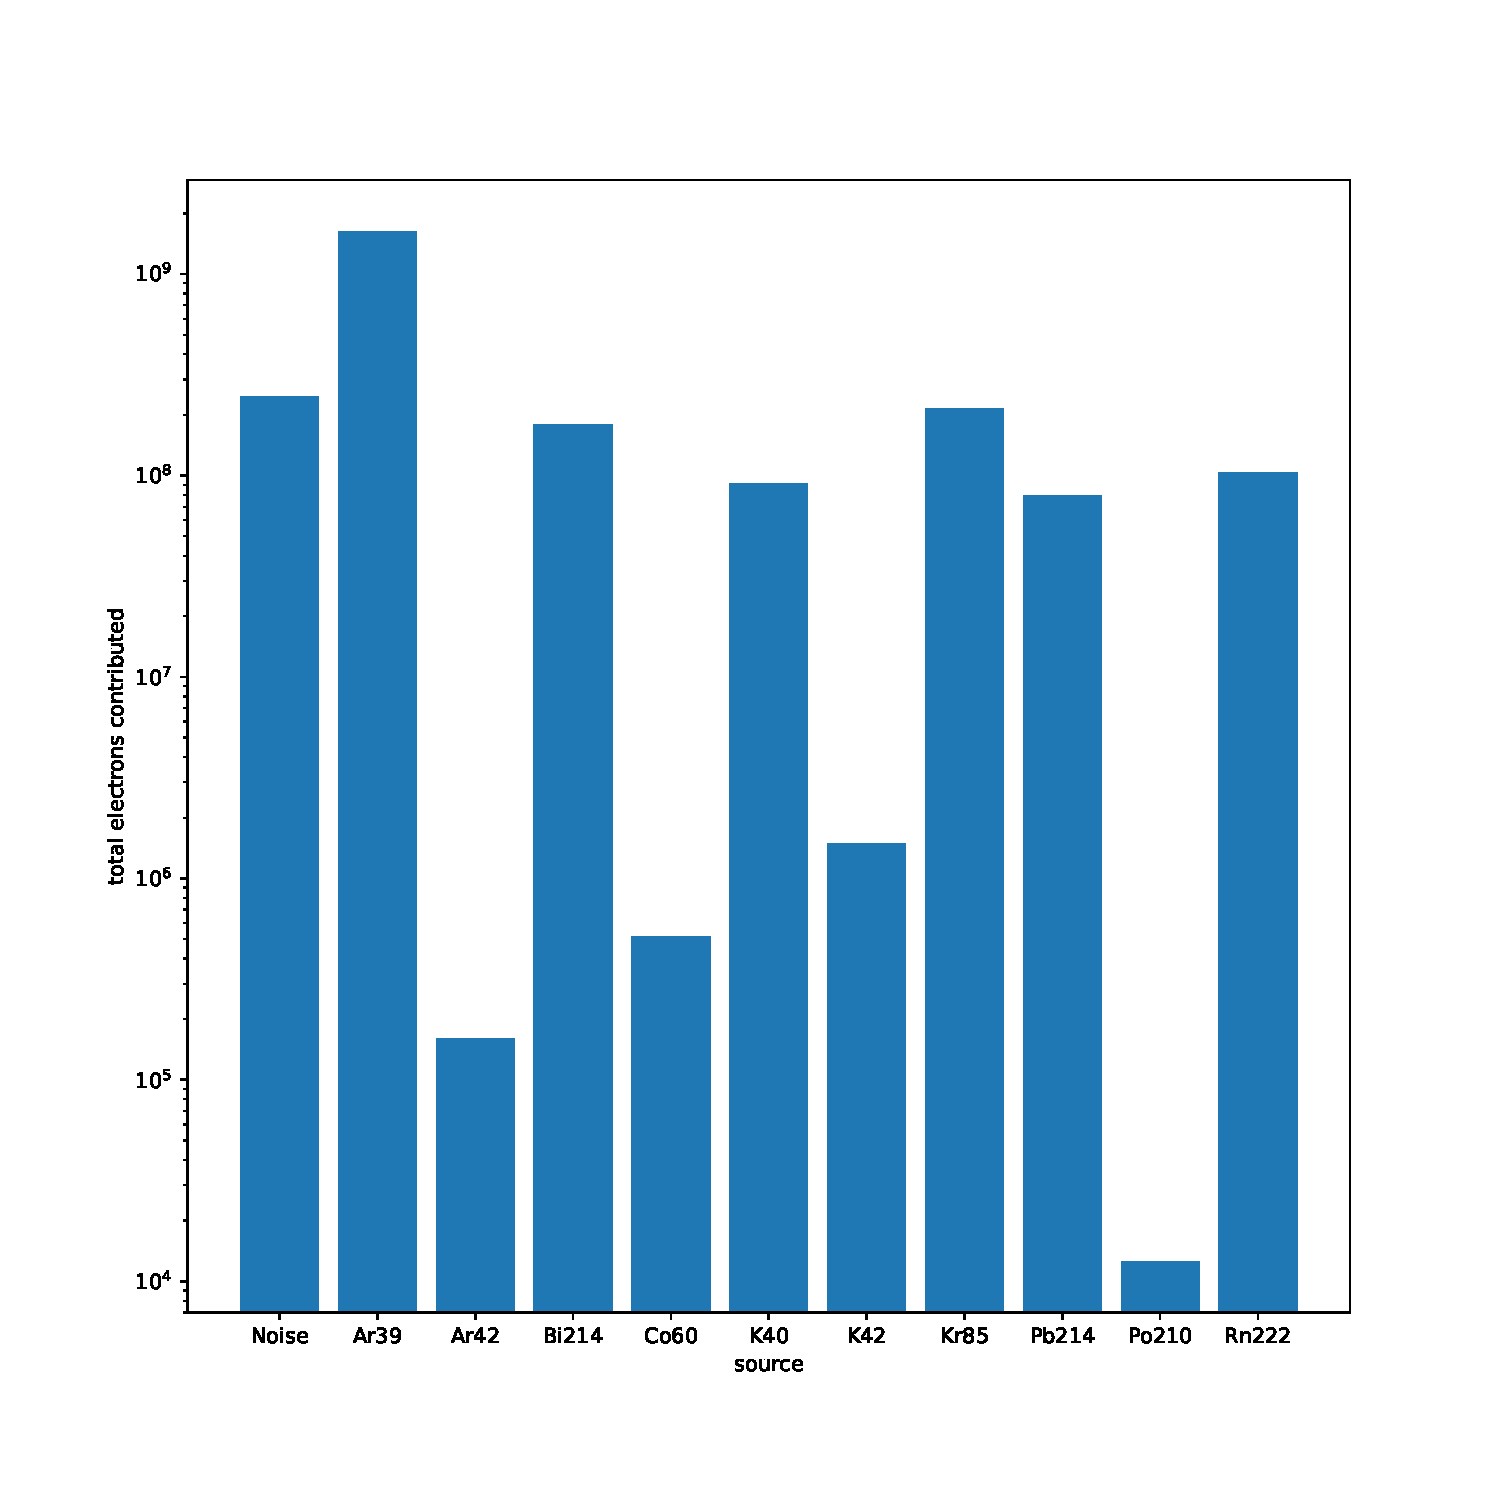
\includegraphics[width=\textwidth]{images/sim_electron_contribution_log.pdf}
  \caption{Contribution of total electrons.}
\end{subfigure}%
\begin{subfigure}{.5\textwidth}
  \centering
  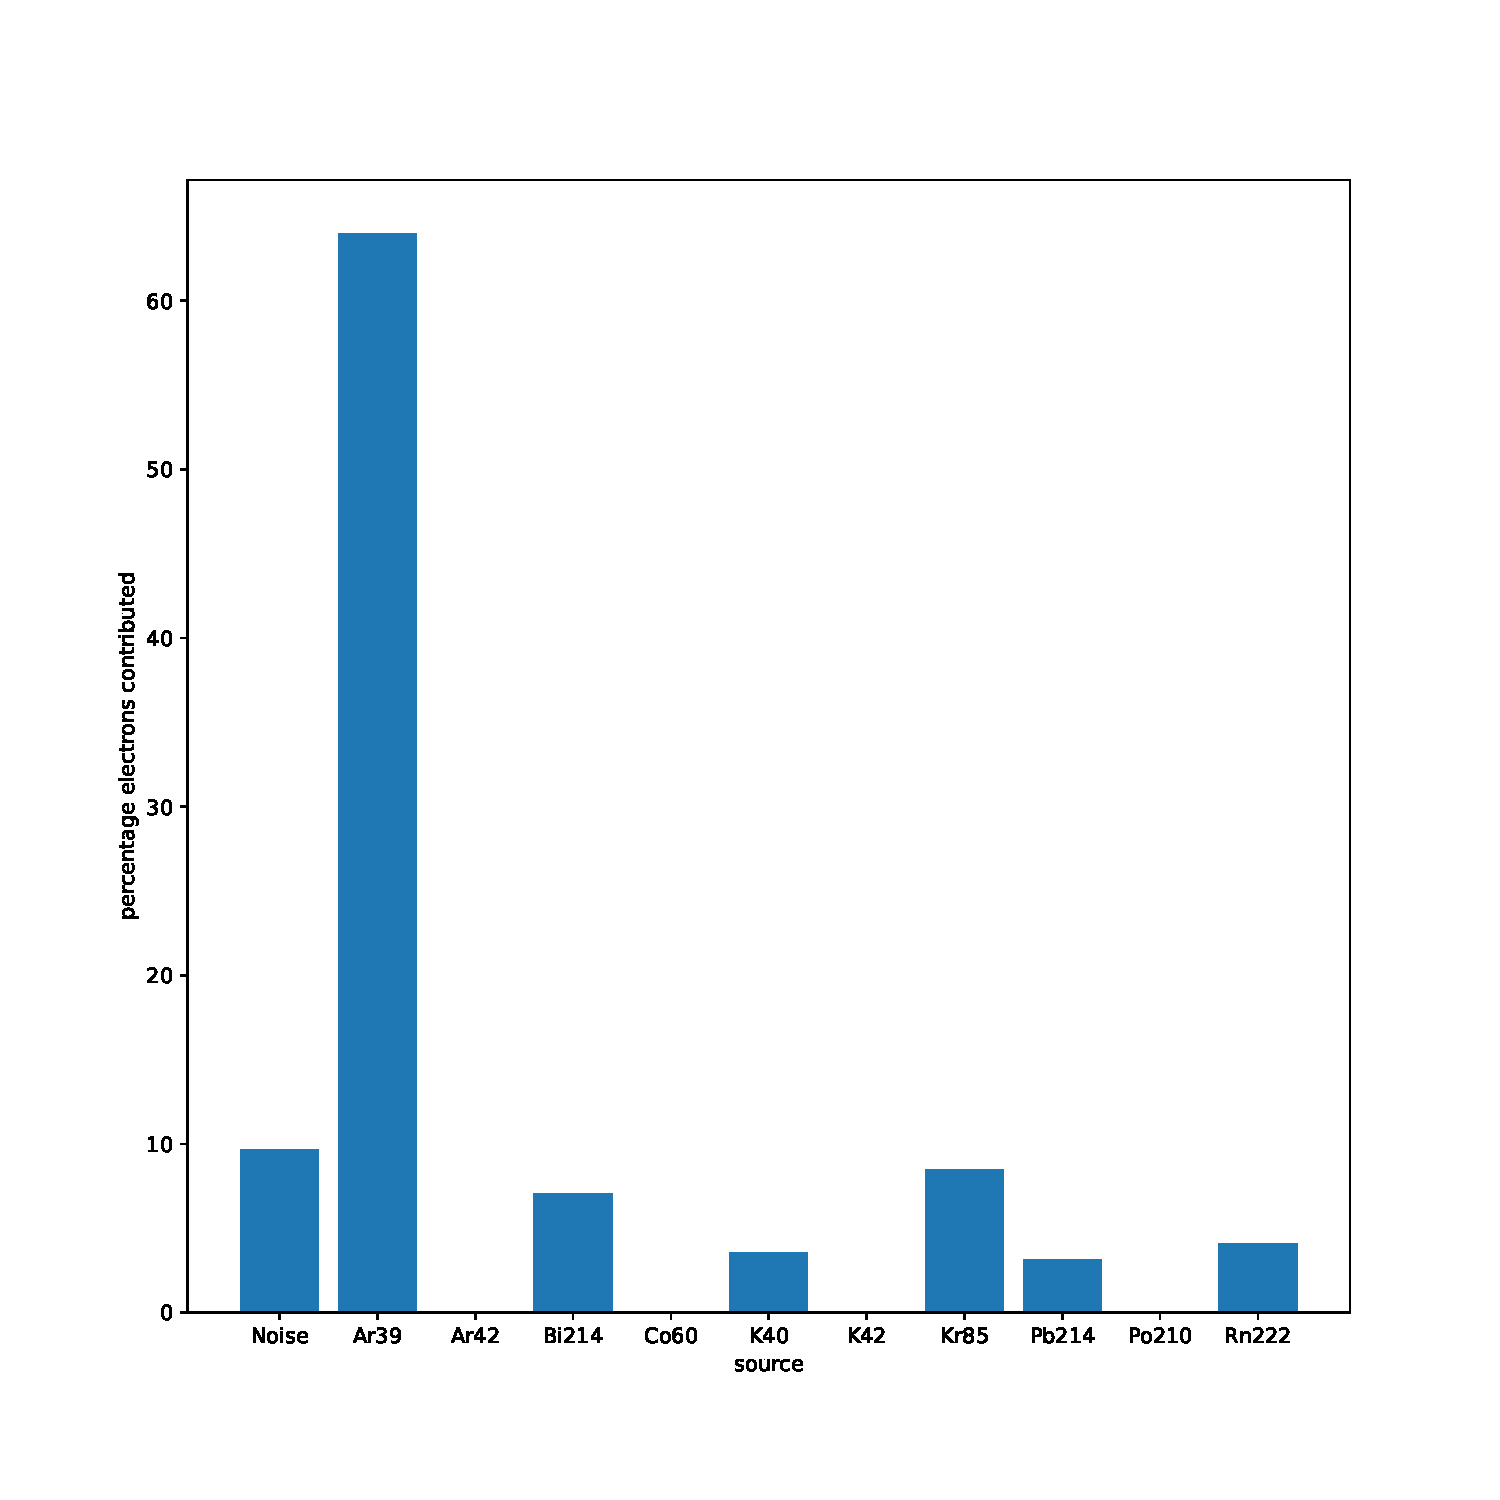
\includegraphics[width=\textwidth]{images/sim_electron_contribution_percent.pdf}
  \caption{Contribution of electrons by percentage.}
\end{subfigure}
\caption{Both figures indicate a comparison of the amount of electrons deposited on all pixels in the tile shown in Figure~\ref{fig:reference_input_noise}.
Plot (A) represents the total number of electrons on a log scale.
As expcted, $^{39}$Ar contributes the majority of background charge.
The leakage current used is 10~\unit{aA}, and represents about 10\% of the total contribution of electrons.
This implies that leakage currents from the front circuit which are $\approx 100$~\unit{aA} will contribute nearly as much electrons to the steady-state RTDs as the radiogenic backgrounds.
}
\label{fig:compare_electron_contribution}
\end{figure}

%%%%%%%%%%%%%%%%%%%%%%%%%%%%%%%%%%%%%%%%%%%%%%%%%%%%%%%%%%%%%%%%%%%%%%%%%%%%%%%%
%%%%%%%%%%%%%%%%%%%%%%%%%%%%%%%   Part 2   %%%%%%%%%%%%%%%%%%%%%%%%%%%%%%%%%%%%%
%%%%%%%%%%%%%%%%%%%%%%%%%%%%%%%%%%%%%%%%%%%%%%%%%%%%%%%%%%%%%%%%%%%%%%%%%%%%%%%%
\section{Neutrino Beam Studies}~\label{sec:neutrino_studies}

Here we discuss the implementation of the digital framework within the high energy regime.
For this we use as an input neutrino events from the Long-Baseline Neutrino Facillity (LBNF)~\citep{dune_cdr_2016_arxiv} and take the unoscillated flux of neutrinos which were used in~\citep{dune_2021_near_detector_cdr}.
These neutrino flux are simulated using GENIE~\citep{Andreopoulos:2009rq}, v2.12.10.
The interaction distributions for both the forward and reverse horn current directions are shown in Figure~\ref{fig:neutrino_interaction_flux}.

We do not perform any calculation involving the oscillation on the input neutrino flux.
The reason for this is that the digital back-end should be able to fully record data from all possible $\nu_{l}$ events regardless of interaction type, not only the intended $\nu_{e}$ appearance spectra.
It is equally important for a future readout to be able to correctly tag noise ($\nu_{\mu}$, or $\nu_{e}$ from the beam, etc.).
For example, sensitivity to mass ordering and CP violation rely on the abiility to measure $\nu_{\mu}$ disappearance in addition to the $\nu_{e}$ appearance.

What will be shown in the upcomming sections is that capability of the digital back-end depends on the energy deposited in the volume of the LAr.
By the virtue that oscillations change only the flavor (not the energy) of the $\nu$, the constraints of the back-end do not depend on if more (or less) $\nu_{e}$ are measured compared to $\bar{\nu_{e}}$, provided the back-end is capable of fully measuring both events.
Furthermore, by using the unoscillated flux of the neutrinos at the near detector, the neutrinos will be of necessarily higher energy than the expected flux at the far detector.
The use of high energy helps in establishing what we will show as the upper-bound for the required local and remote FIFO depths for each ASIC.

\begin{figure}[]
\centering
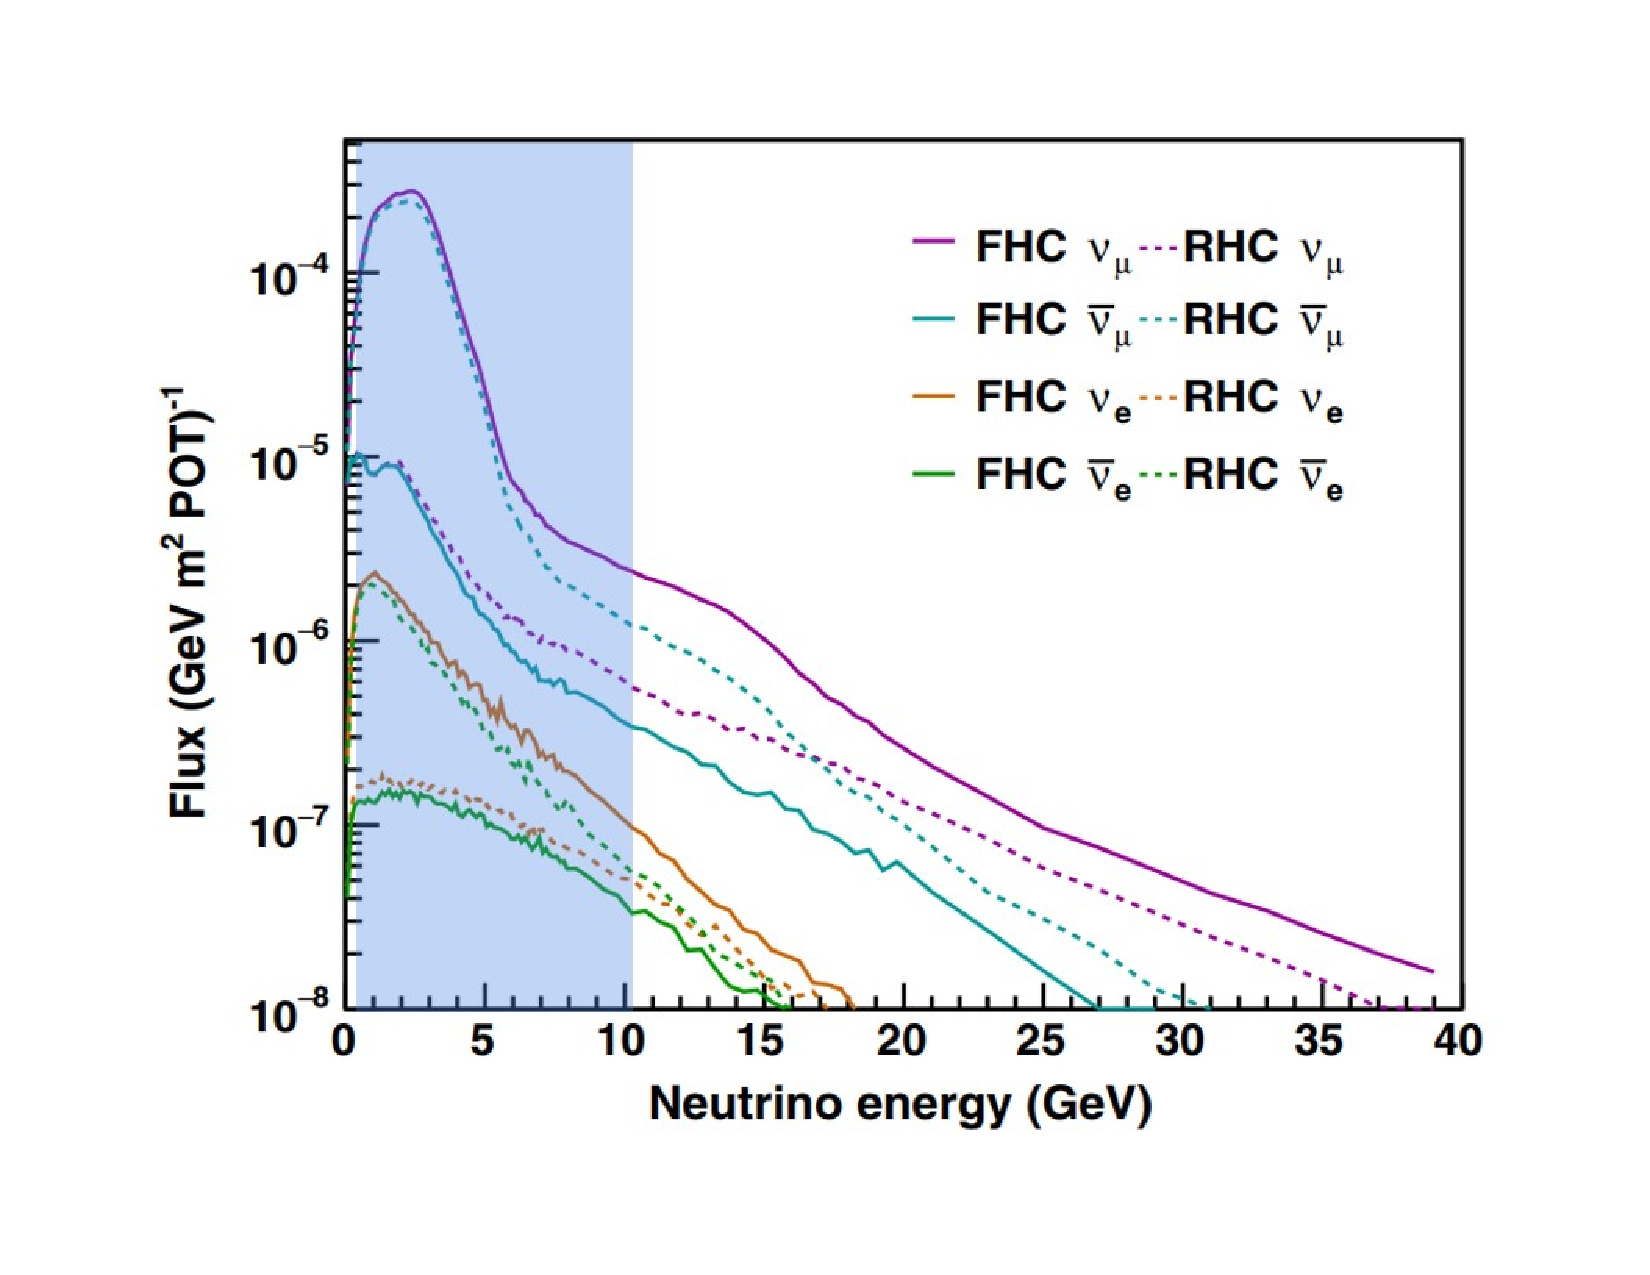
\includegraphics[width=\textwidth]{images/dune_flux_energy_range.pdf}
\caption{Flux spectrum of neutrinos from the neutrino beam used in this study. This figure is taken from~\cite{electron_flux_image_2020}. 
Highlighted in blue is the reconstructed energy range of neutrinos that are used to seed the interaction with the APA LAr's volume.}
\end{figure}~\label{fig:neutrino_flux}

\begin{figure}[]
\centering
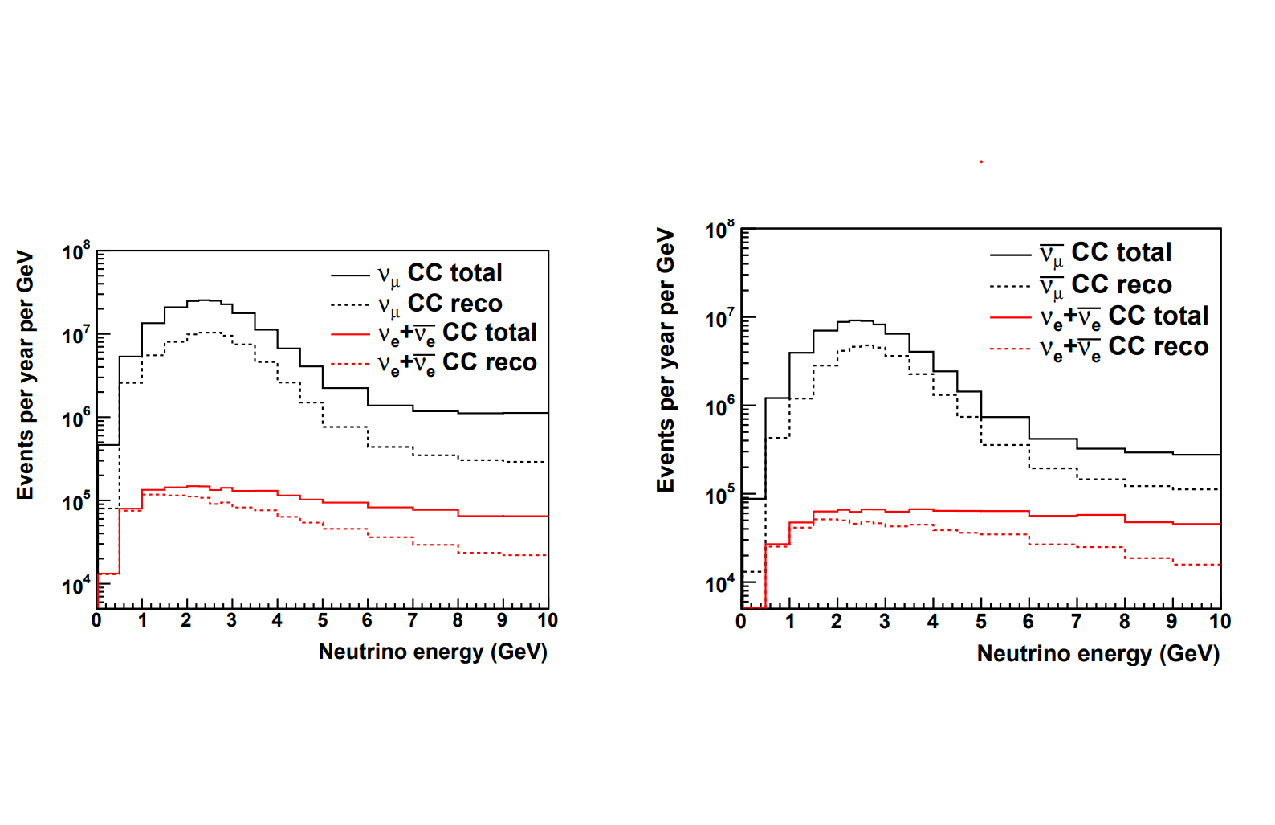
\includegraphics[width=\textwidth]{images/dune_cdr_2021_neutrino_flux.pdf}
\caption{Rate of CC neutrino interactions based on flavor as a functino of true neutrino energy.
Figure is taken directly from~\citep{dune_2021_near_detector_cdr}.
Right is shown the neutrino interaction distribution for the forward horn current.
The left image is for the reverse horn current.
Both images assume an average exposure rate of 1.2 MW from LBNF beam.}
\end{figure}~\label{fig:neutrino_interaction_flux}


\subsection{Neutrino Event Parameters}

Table~\ref{table:neutrino_params} describes the parameters of each input for the simulation.
The parameters used to vary the tiles for these neutrino input energies are shown on Table~\ref{table:tile_params}.

The Q-Pix readout presented here is designed for use in a LArTPC at the scale of DUNE-FD 10kT module~\ref{sec:dune}.
In order to test what kinds of requirements this readout will need we use high energy neutrino interactions as discussed in Section~\ref{sec:neutrino_studies}.
The different selection parameters for each event are neutrino flavor, neutrino energy, horn current direction, Z-position vertex position, and source neutrino momentum direction ($\theta_{z})$.
We define the beam direction (the direction parallel to the surface of the APA) as $\theta_{z} = 0$.
The X and Y positions are held constant for all interactions, at X = 120~\unit{cm} and Y = 3200~\unit{cm}.
The coordinate system we use, as well as a slice of the APA within a module are shown in Figure~\ref{}.

The LBNF beam is not the only source of high energy particles DUNE will detect.
Other high energy ($\simeq 10$~\unit{GeV}) interactions may come from other sources.
These other high energy events (such as nucleon decay, cosmic neutrinos) may also deposit energy on~\unit{GeV} scales per interaction.
These sources may interact with their net momentum vector pointing in any direction.
For this reason we also test $\nu_{e}$ and $\nu_{\mu}$ interactions at $\theta_{z} \pm$ 90~\unit{\degree}; this direction causes the secondary ionizing particles to carry momentum along the direction parallel to the pixel's surface normal.
These two momentum directions, though unphysical for beam interactions, still present possible interactions types within the scope of DUNE's propossed physics program~\citep{DUNE_TDRv3_Abi_2020}.

\begin{table}
\begin{center}
\begin{tabular}{|| p{30mm} | p{30mm} | p{90mm} ||}
 \hline
 Name & Values & Relation \\ [0.5ex]
 \hline\hline
  $\nu_{l}$ & $\nu_{e}$, $\bar{\nu_{e}}$, $\nu_{\mu}$, $\bar{\nu_{\mu}}$ & Oscillation measurements require sensitivity to measurements for both $\nu_{e}$ appearance, and $\nu_{\mu}$ disappearance.\\
 \hline
  $\nu_{l}$ Energy & 0.25~\unit{GeV} to 10~\unit{GeV}, in steps of 0.25~\unit{GeV} & neutrino energy determines output secondary energy, which causes more resents and directly affects buffer depths. \\
 \hline
  Horn Current & Forward and Reverse & Beam horn current direction affects neutrino flux, as shown in Figure~\ref{fig:neutrino_flux}. Additionally, mass heirarchy measurements (according to the MSW effect~\citep{Smirnov2004TheME}) require difference in measurements of appearance probability for $\nu_{e}$ and $\bar{\nu_{e}}$. \\
 \hline
  Z-position & 10~\unit{cm}, 80~\unit{cm}, 180~\unit{cm}, 280~\unit{cm}, 350~\unit{cm}  & Interaction z-position above the anode plane. Interactions which happen further from the collection plane have more time to diffuse or recombine. \\
 \hline
  $\theta_{z} $ & 0\unit{\degree}, $\pm$2\unit{\degree}, $\pm$90\unit{\degree} & Different momentum angles are different Z-positions, in general, direct ionized particle tracks within the active volume. \\
 \hline
\end{tabular}
\caption{The different neutrino simulation parameters which are passed into Geant4 based simulation.
  The original interaction products are generated using GENIE~\citep{Andreopoulos:2009rq} v2.12.10.
  The output products of the neutrino interaction produced from GENIE are then configured using the different parameters described above.
  We select $\nu_{l}$ events for different energies in bin-widths of 250 MeV; We follow the same bin width as is done in~\citep{DUNE_FD_TDRv2_2020} for their neutrino oscillation analysis.
  A selection of 100 events for each $\nu_{l}$ is taken within each energy bin, for a total of 3900 $\nu_{l}$ events for each horn current direction, z-position, and $\theta_{z}$ selection.
  Since there are two current directions, four $\nu_{l}$, five z-positions, and five $\theta_{z}$ positions, a total of 780,000 neutrino events are simulated.
}
\end{center}
\end{table}
~\label{table:neutrino_params}

%% fig example neutrino event
% image example of a full event with rotations
\begin{figure}
\centering
\begin{subfigure}{.5\textwidth}
  \centering
  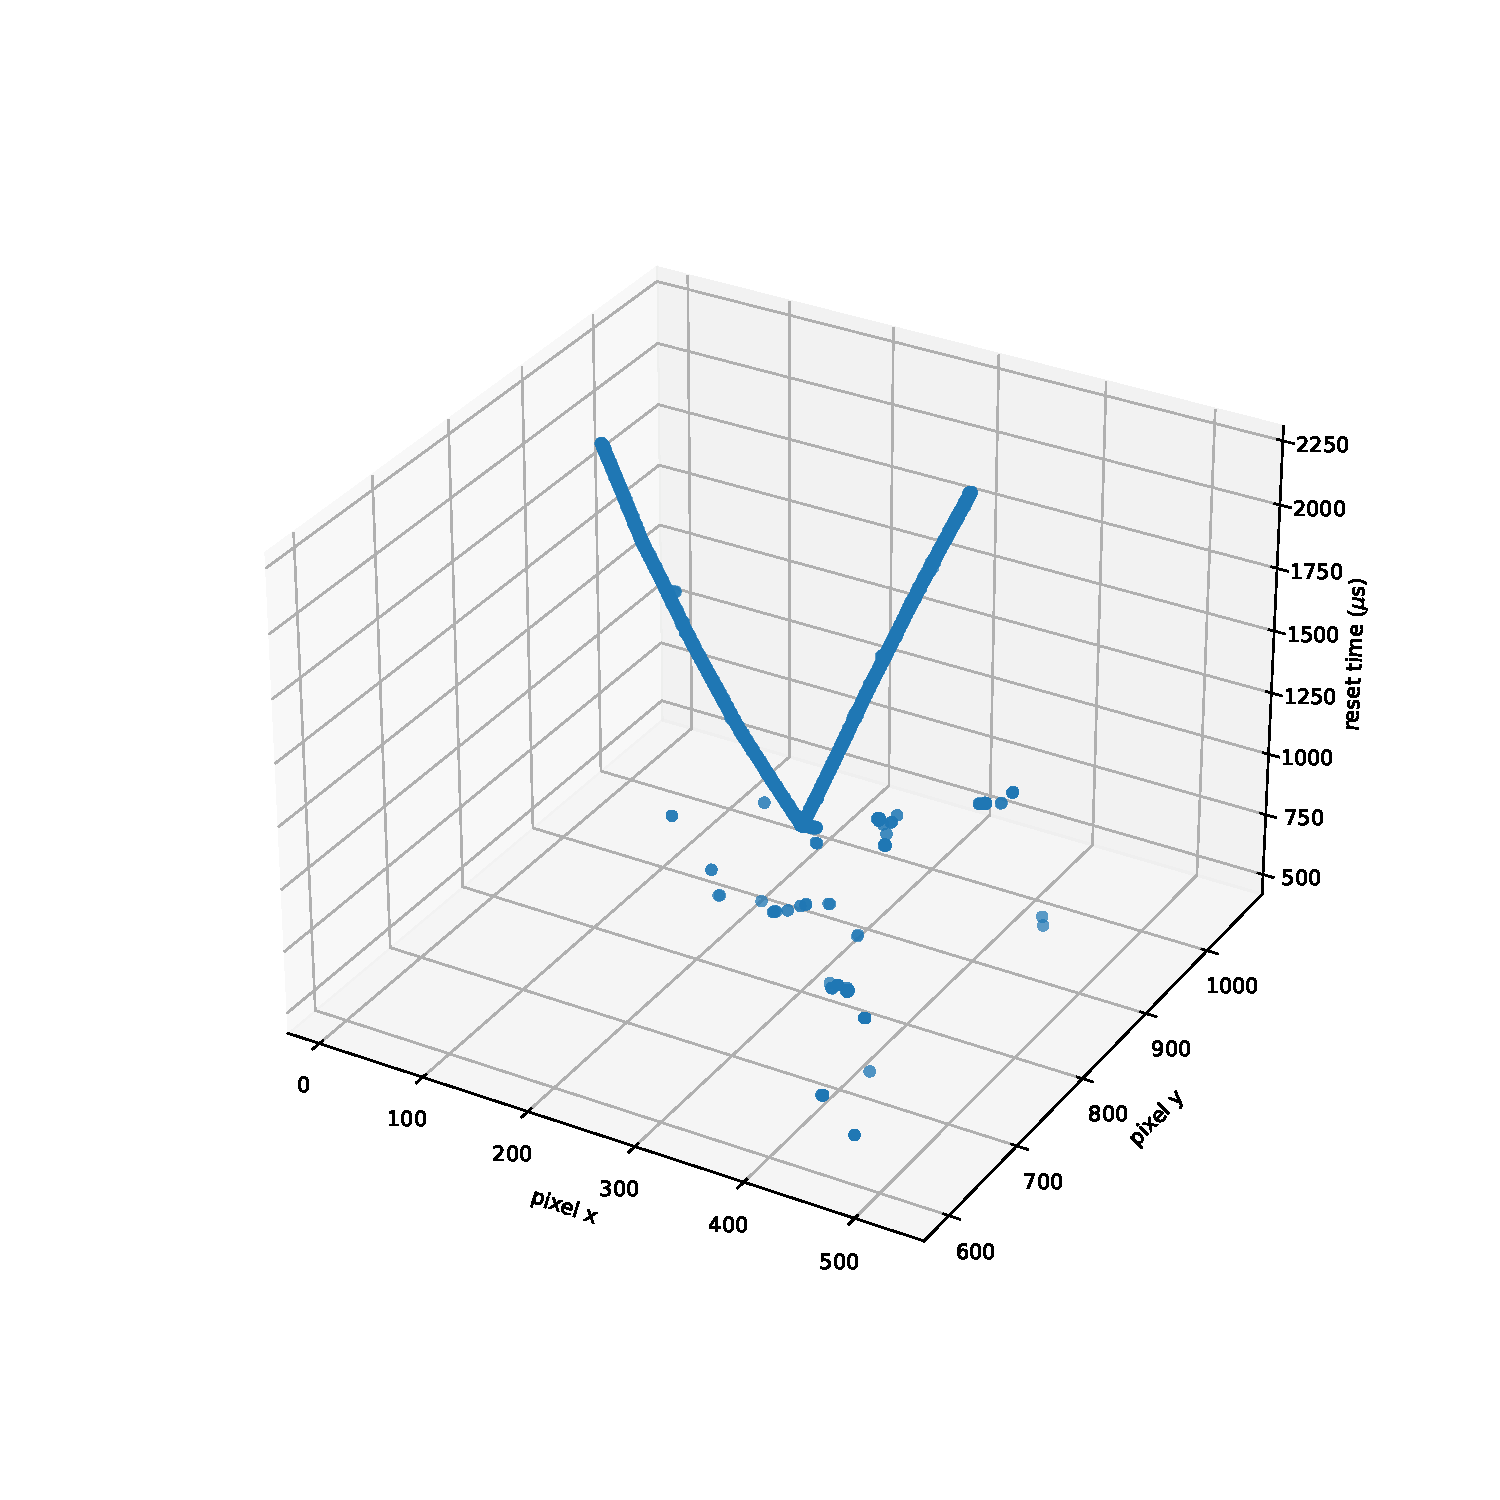
\includegraphics[width=\textwidth]{images/example_zdir_scatter.pdf}
  \caption{$\theta_{z} = +90$\unit{\degree}}
\end{subfigure}%
\begin{subfigure}{.5\textwidth}
  \centering
  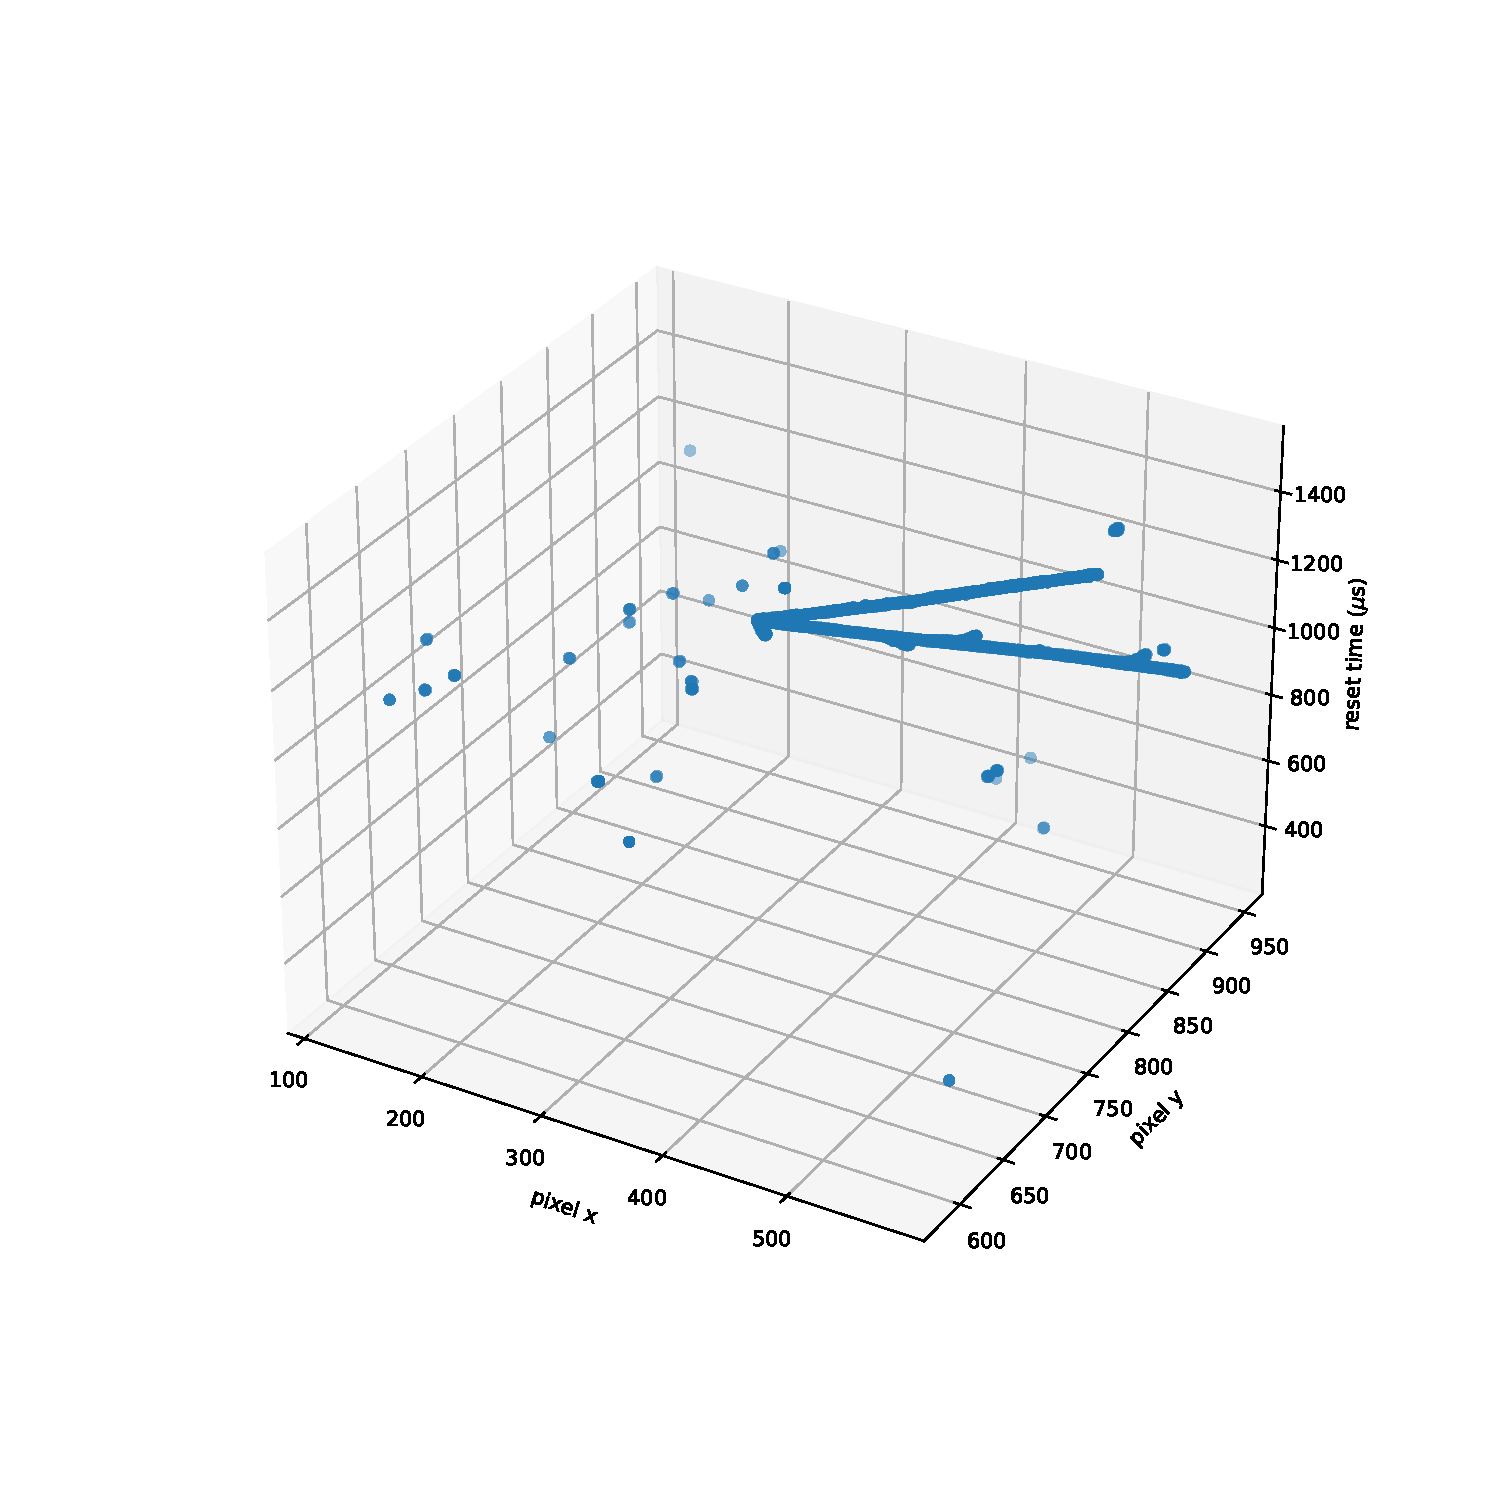
\includegraphics[width=\textwidth]{images/example_xdir_scatter.pdf}
  \caption{$\theta_{z} = 0$\unit{\degree}}
\end{subfigure}
\caption{Same $\nu_{e}$ interaction at Z-position $= 180 cm$, which is in the middle of the drift length of the APA.
Image (A) has the incident $\nu_{e}$ momentum rotated upwards ($\theta_{z} = +90$\unit{\degree}).
Image (B) has the incident $\nu_{e}$ had momentum along the beam direction ($\theta_{z} = 0$\unit{\degree})y.
Since there are five different z-positions, and five different $\theta_{z}$ values, each of the 3900 $\nu_{l}$ interactions are repeated 25 times.
These two plots show two of those 25 examples.
}
\label{fig:compare_integral}
\end{figure}

\begin{figure}[]
\centering
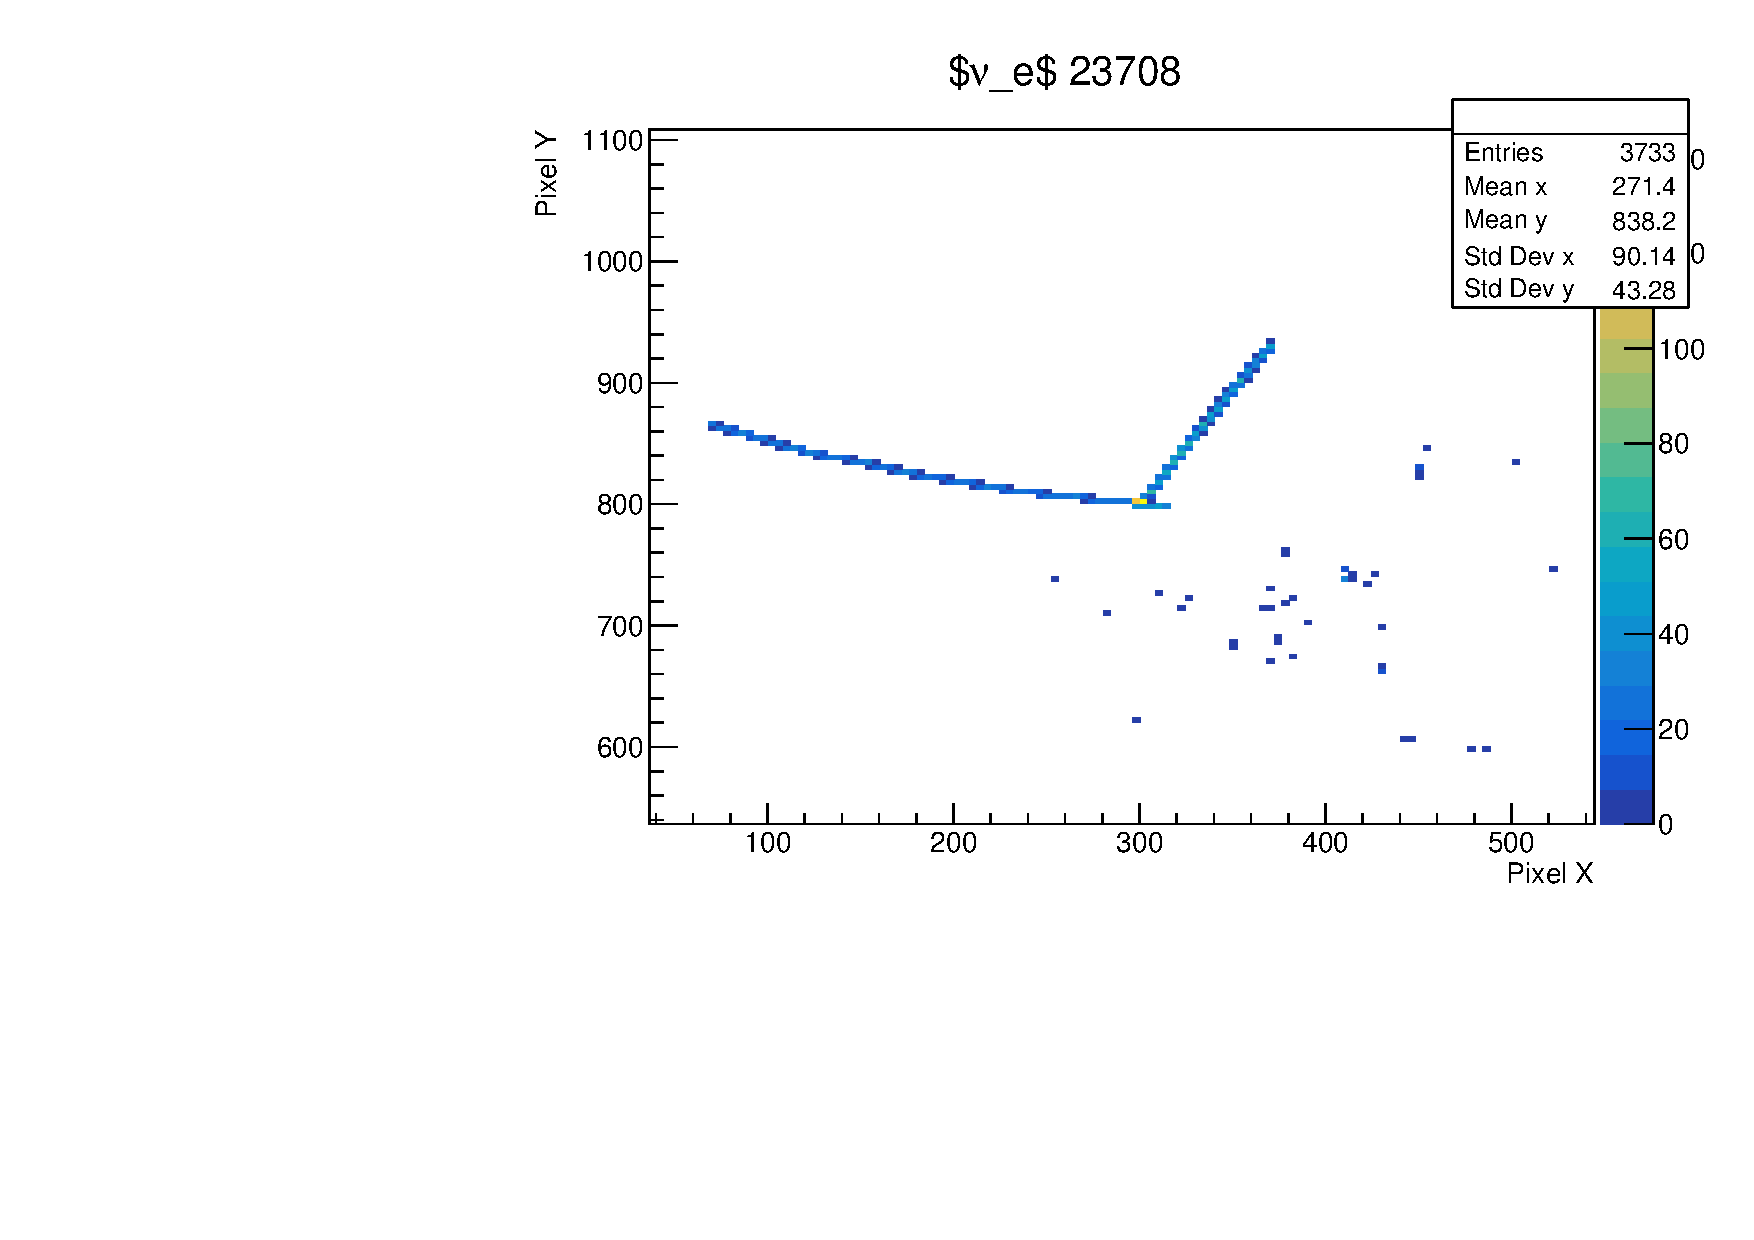
\includegraphics[width=\textwidth]{images/electron_fhc_23708_event.pdf}
\caption{The same $\nu_{e}$ event as the one shown in Figure~\ref{fig:compare_integral}-(A).
The plot is zoomed into to the region of interest where the bin widths represent the pixels dimensions in the collection plane.
The energy of this $\nu_{e}$ was 546.1~\unit{MeV}, and considering that each reset requires 0.1475~\unit{MeV}, the maximum number of resets this event could produce is $\approx 4368$.
The histogram records 3733 total resets.
The most active pixel received 144 resets.
When the pixels are binned into ASICs (4$\times$4 pixels) the maximum number resets an ASIC received is 347.
}
\end{figure}~\label{fig:asic_th2i_electron_fhc_event}

\subsection{Neutrino Event Results}

Every simulated neutrino interaction generates some number of resets which are collected onto the pixel plane.
The purpose of the study explored by the parameters described in Table~\ref{table:neutrino_params} is to investigate the charge resets these interactions produce; we pay particularly close attention to ASICs where the number of resets (energy deposited) is the largest in a given event.

We bin the maxmimum number of resets in a 4$\times$4 pixel array, or ASIC, for every neutrino event.
The first plot Figure~\ref{fig:example_asic_integral_value_constTheta}-(A) shows a $\nu_{e}$ event and Figure~\ref{fig:asic_th2i_electron_fhc_event} shows these resets binned into pixels.

This value represents the required local FIFO depth in order to capture all of the resets produced by this event.
 
%% example integral of ASIC buffer depths with constant theta
\begin{figure}
\centering
\begin{subfigure}{.5\textwidth}
  \centering
  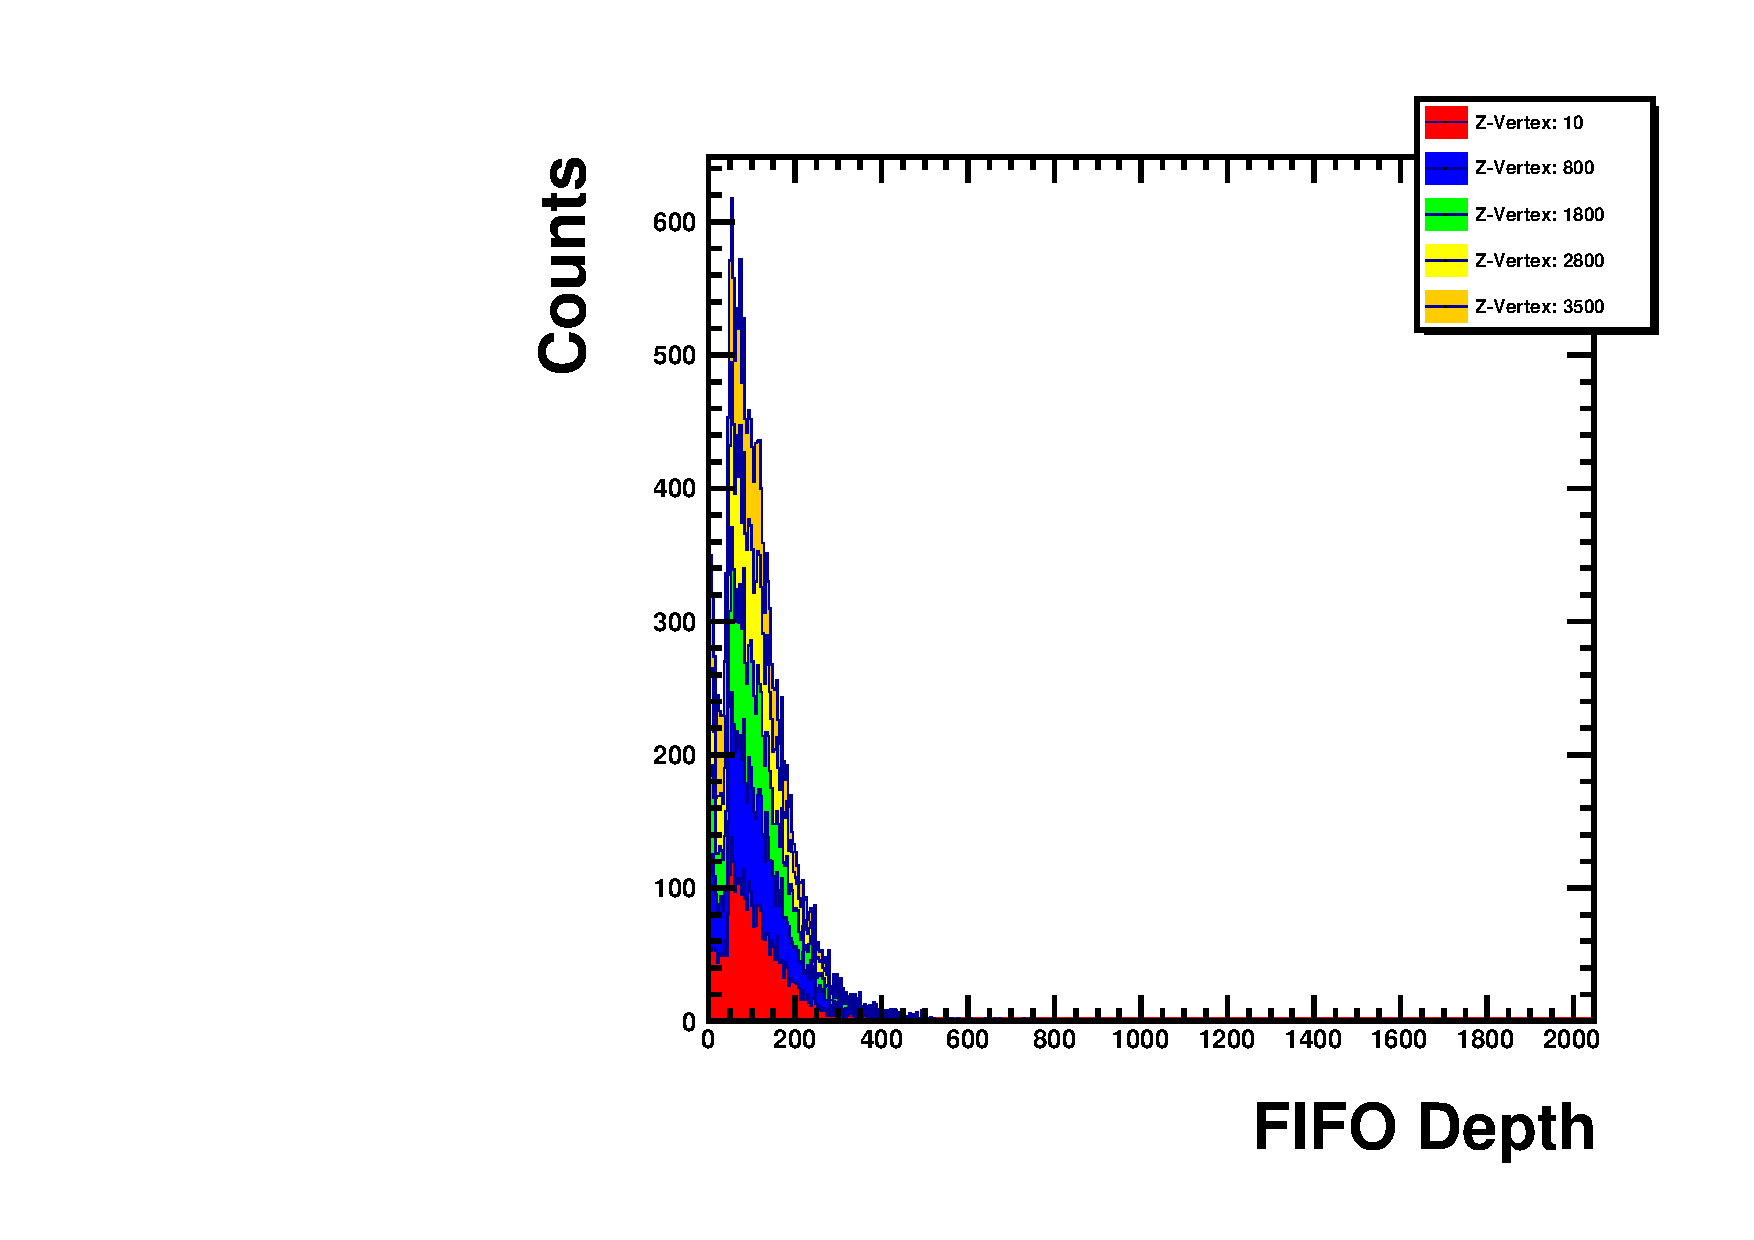
\includegraphics[width=\textwidth]{images/Const_Theta0_ASIC_stack_integral_pdg12_fhc.pdf}
  \caption{ASIC Local FIFO Depths}
\end{subfigure}%
\begin{subfigure}{.5\textwidth}
  \centering
  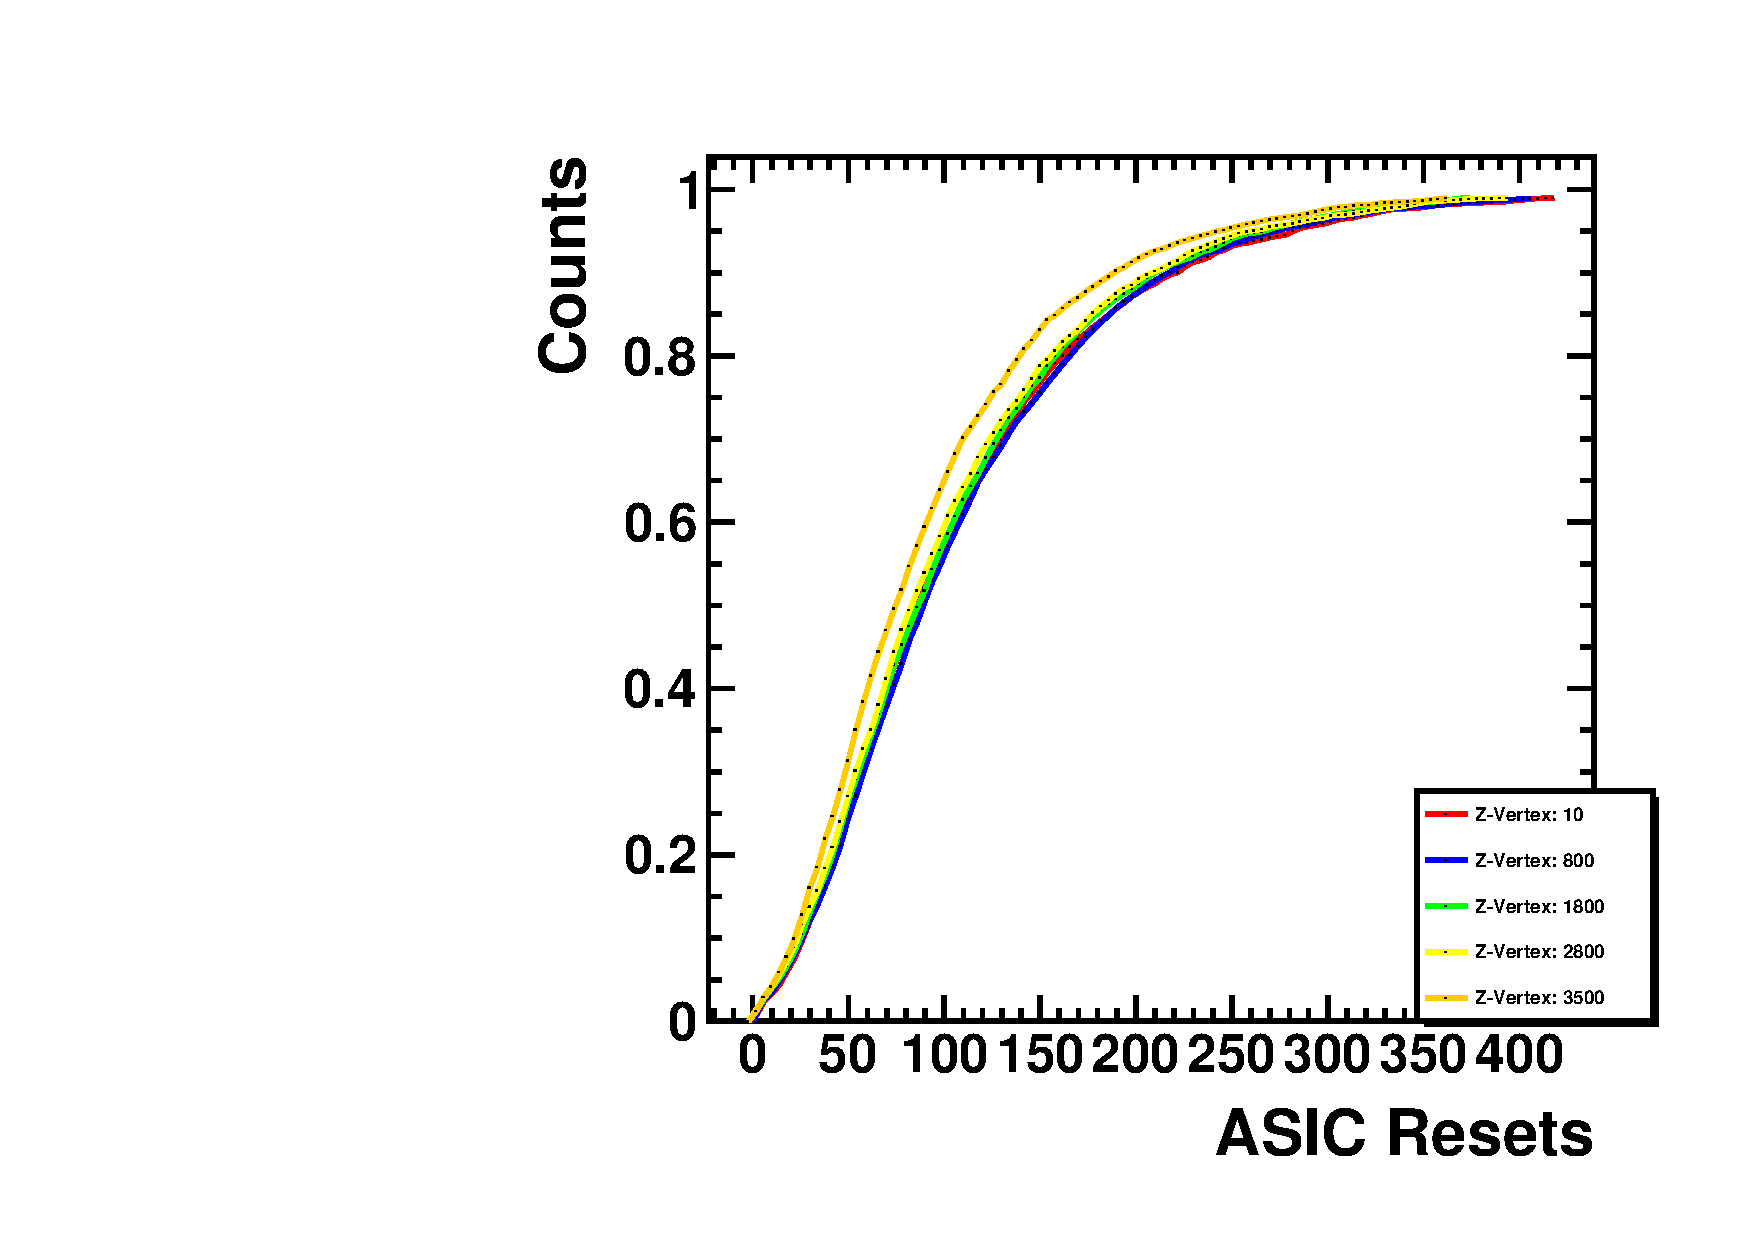
\includegraphics[width=\textwidth]{images/Const_Theta0_ASIC_integral_pdg12_fhc.pdf}
  \caption{Integral of FIFO depths}
\end{subfigure}
\caption{Example $\nu_{e}$ events for different z-position of the vertex with $\theta_{z} = 0$ held constant.
Plot (A) bins the maximum value of local FIFO depth for all 3900 events (energies between 250~\unit{MeV} - 10~\unit{GeV}) for variable z-position and $\theta_{z} = 0$.
Plot (B) shows the running integral for each histogram shown in plot (A).
The integral continues until 99\% of all events are counted, or the integral reaches a value of 3861.
This process is repeated for all 200 possible parameter choices as discussed in Table~\ref{table:neutrino_params}.
}
\label{fig:example_asic_integral_value_constTheta}
\end{figure}


%% example integral of ASIC buffer depths with constant zpos value
\begin{figure}
\centering
\begin{subfigure}{.5\textwidth}
  \centering
  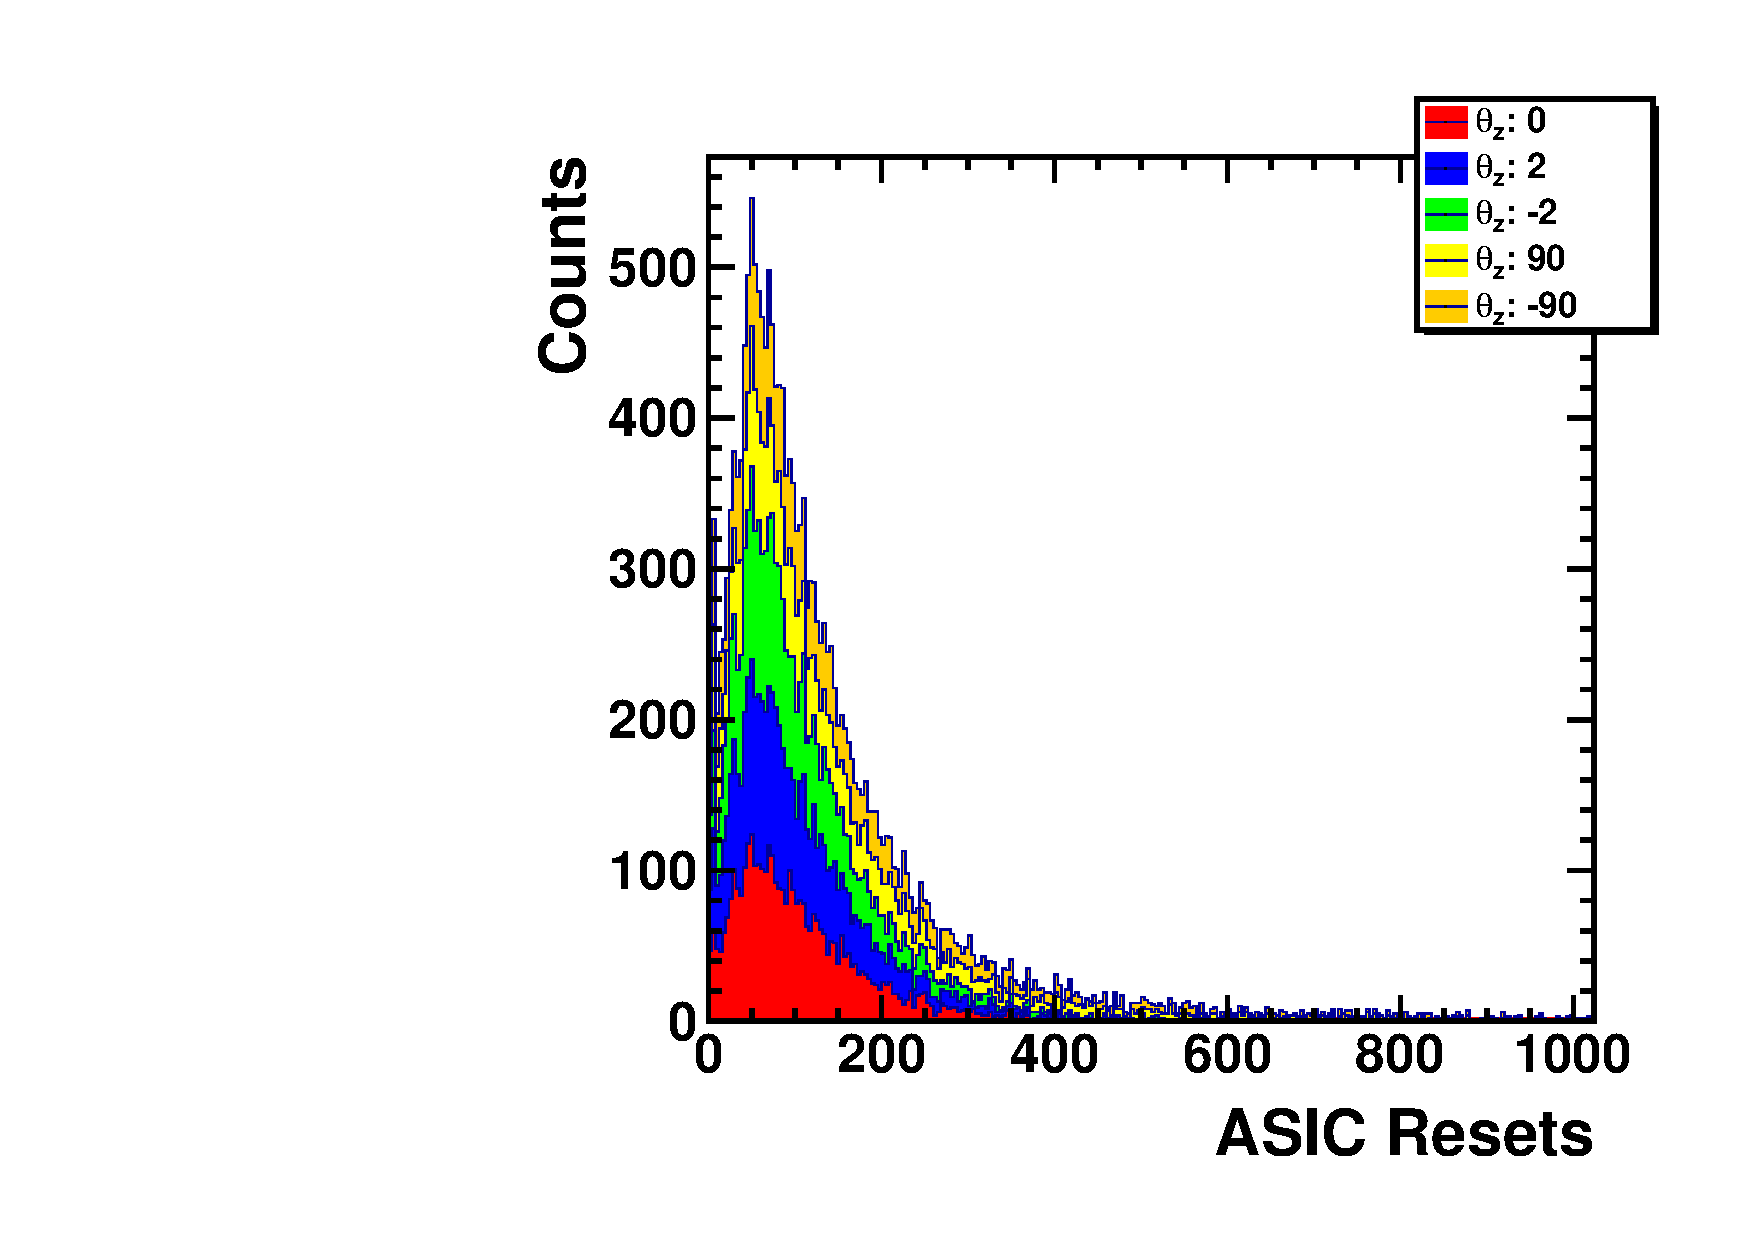
\includegraphics[width=\textwidth]{images/Const_Z180_ASIC_stack_integral_pdg12_fhc.pdf}
  \caption{ASIC Local FIFO Depths}
\end{subfigure}%
\begin{subfigure}{.5\textwidth}
  \centering
  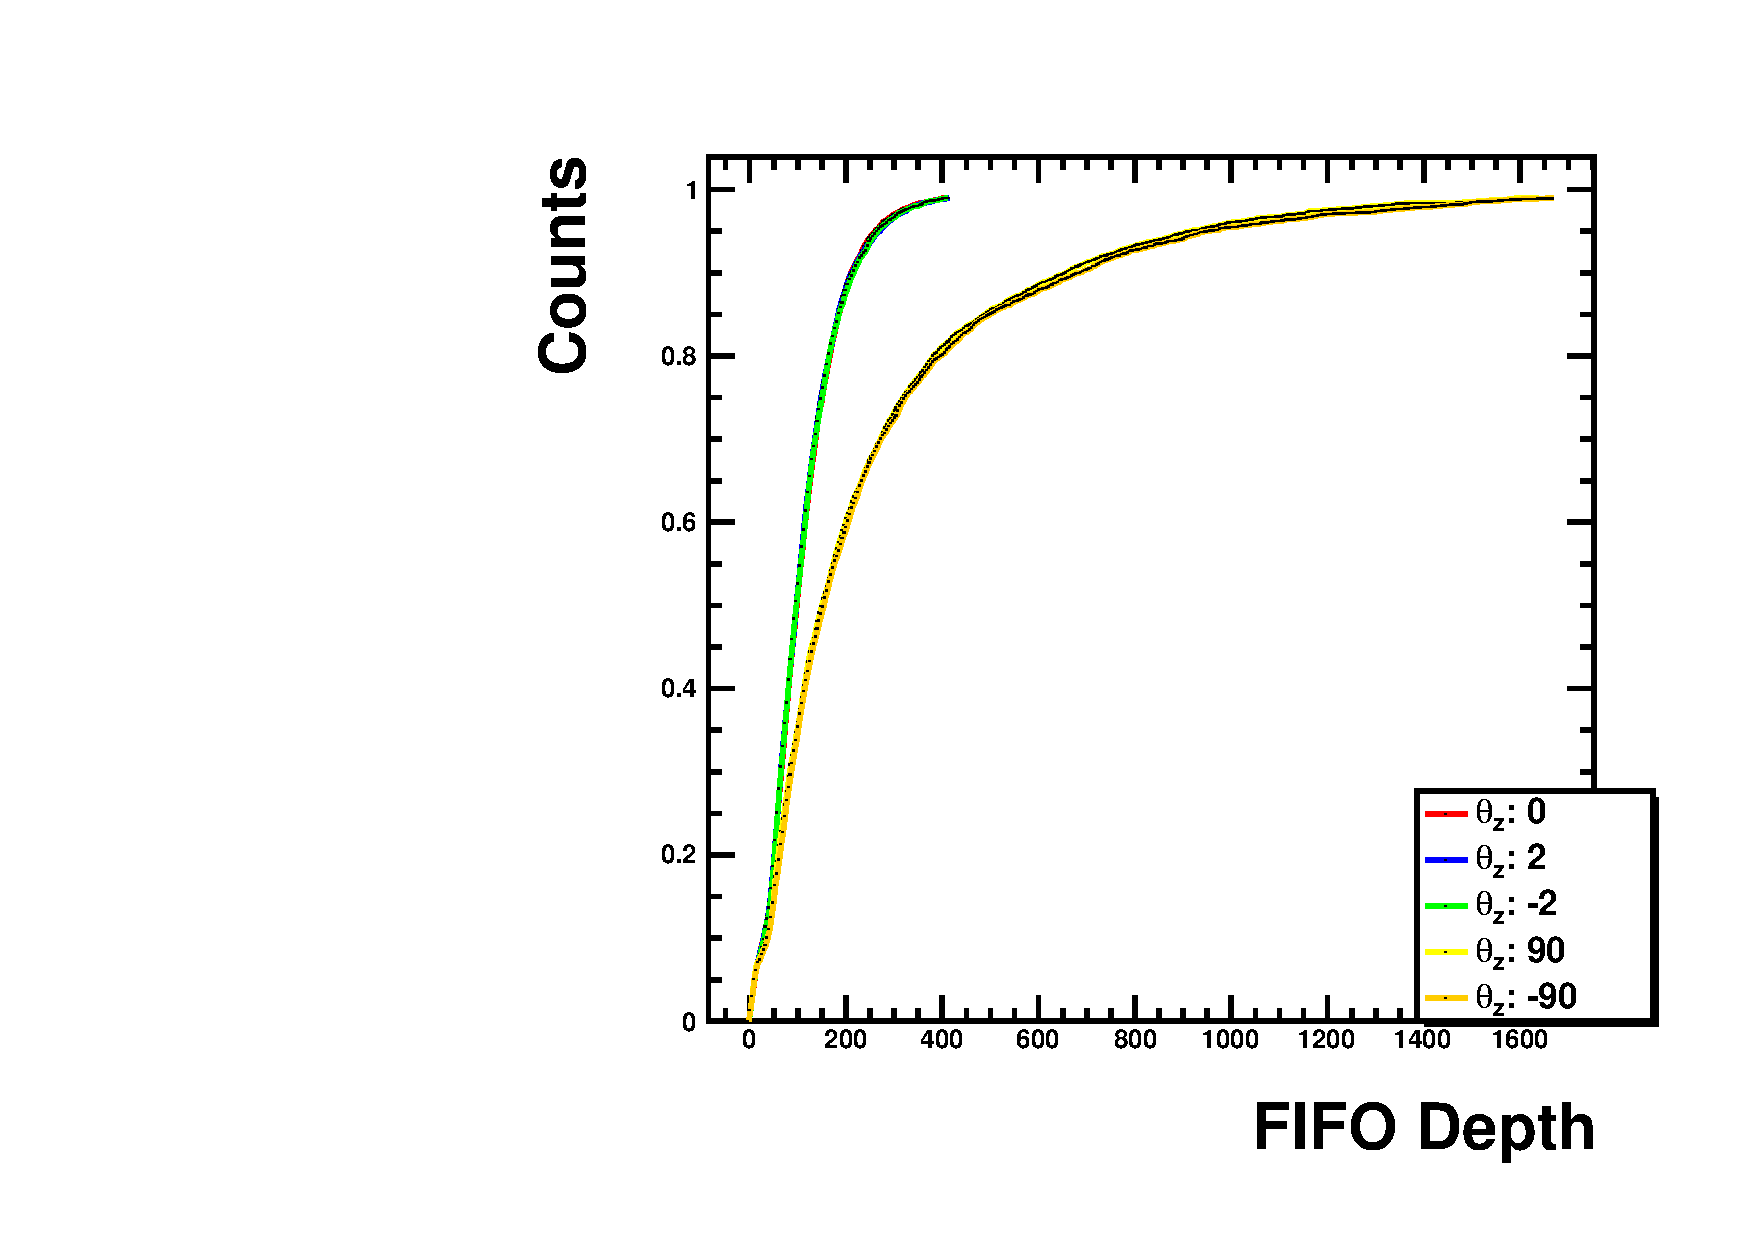
\includegraphics[width=\textwidth]{images/Const_Z180_ASIC_integral_pdg12_fhc.pdf}
  \caption{Integral of FIFO depths}
\end{subfigure}
\caption{Example $\nu_{e}$ events for different $\theta_{z}$ with the vertex held constant with z-position = 180cm.
This is a similar plot to Figure~\ref{fig:example_asic_integral_value_constTheta} with the exception that $\theta_{z}$ is varied and the z-position is held constant at z = 180~\unit{cm}.
A striking difference to note here is the run away effect of the large values of $\theta_{z}$.
}
\label{fig:example_asic_integral_value_constZpos}
\end{figure}

%% energy comparison for different different zpos and theta values
\begin{figure}
\centering
\begin{subfigure}{.5\textwidth}
  \centering
  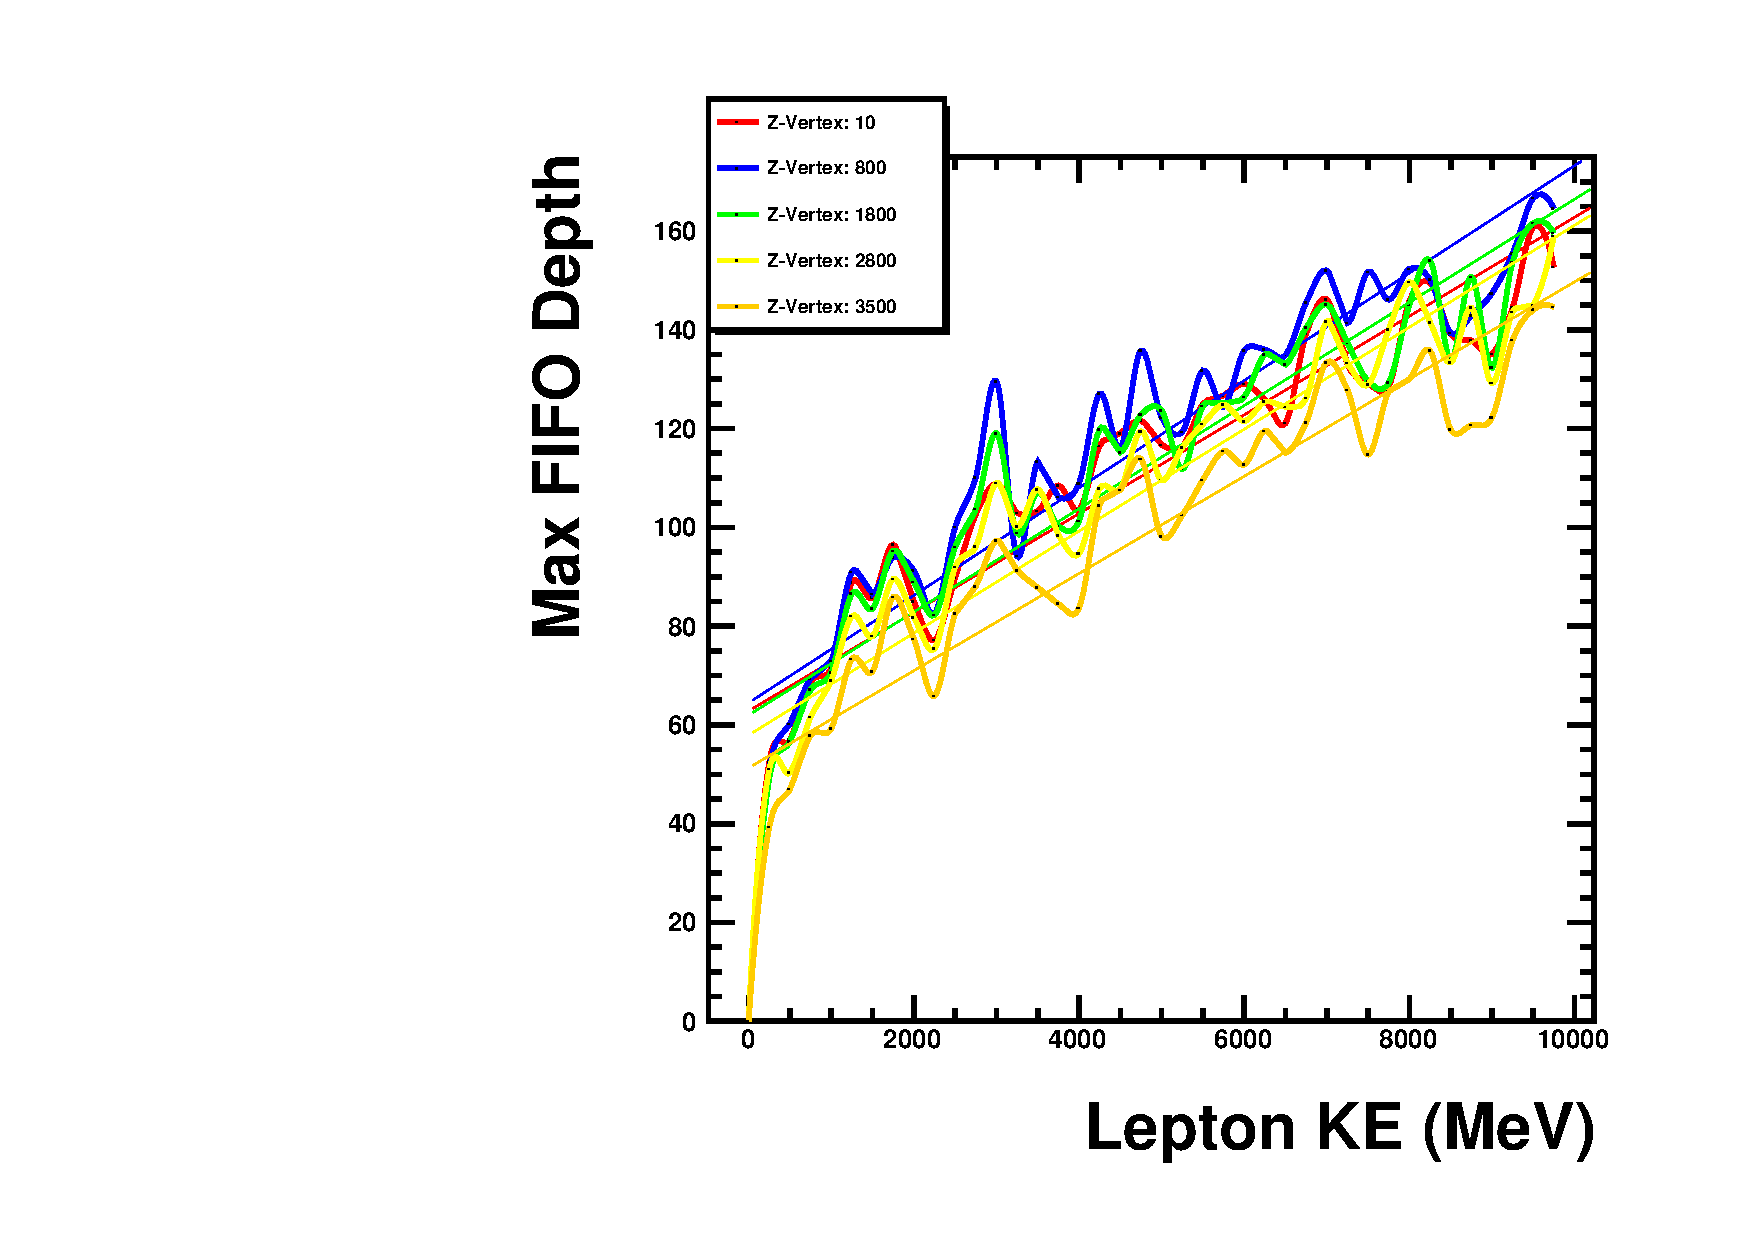
\includegraphics[width=\textwidth]{images/Const_Theta0_ASIC_lepKE_multigraph_pdg12_fhc.pdf}
  \caption{Constant $\theta_{z} = 0$ direction.}
\end{subfigure}%
\begin{subfigure}{.5\textwidth}
  \centering
  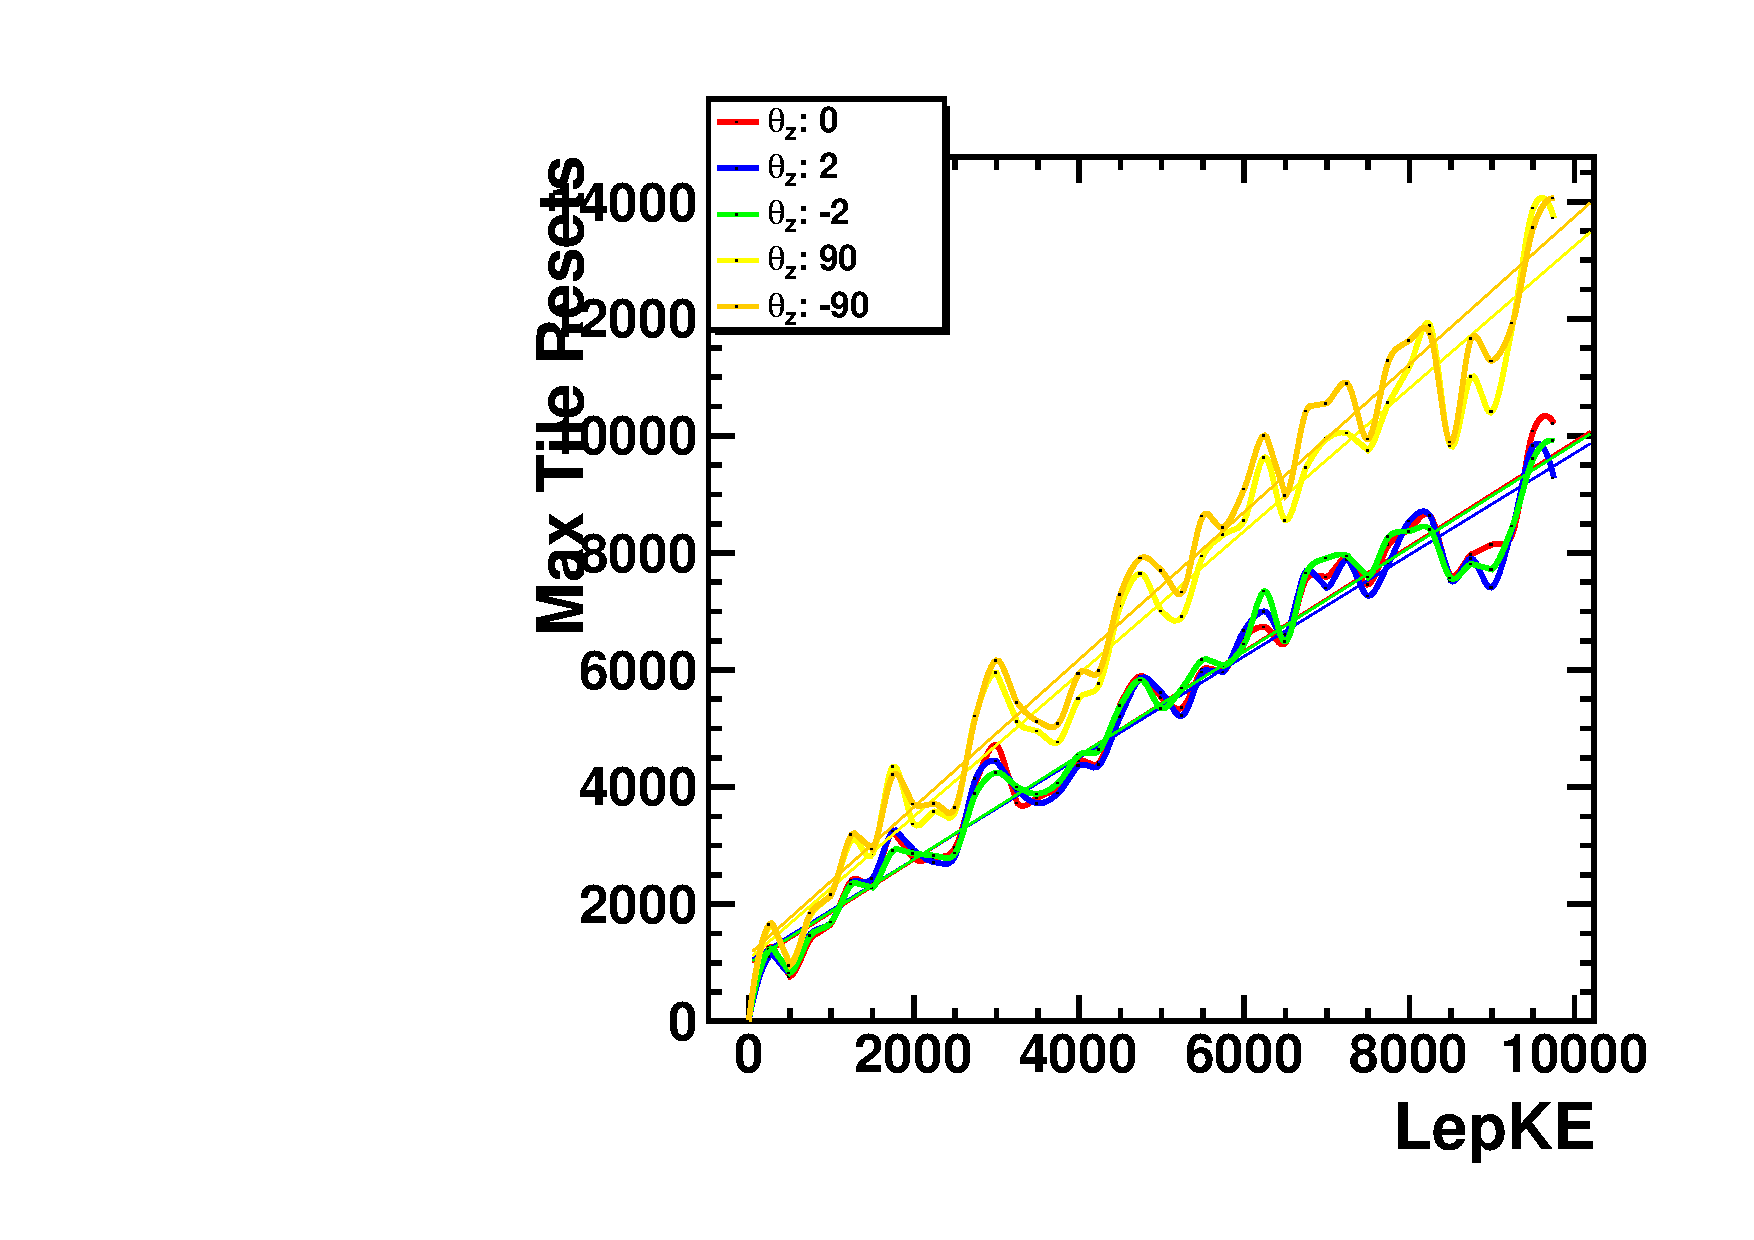
\includegraphics[width=\textwidth]{images/Const_Z180_ASIC_lepKE_multigraph_pdg12_fhc.pdf}
  \caption{Constant Z-Position: $Z = 180~$\unit{cm}.}
\end{subfigure}
\caption{Comparison of Buffer depths as a function of energy for different parameters of $\theta_{z}$ and z-position.
There is a large variance between the true $\nu_{l}$ incident energy and the actual energy deposited in the LAr.
This is the reason why only the means are plotted for each energy bin.
}
\label{fig:example_asic_energy_comparison}
\end{figure}

%% compare energy deposit and lepton energy
\begin{figure}
\centering
\begin{subfigure}{.5\textwidth}
  \centering
  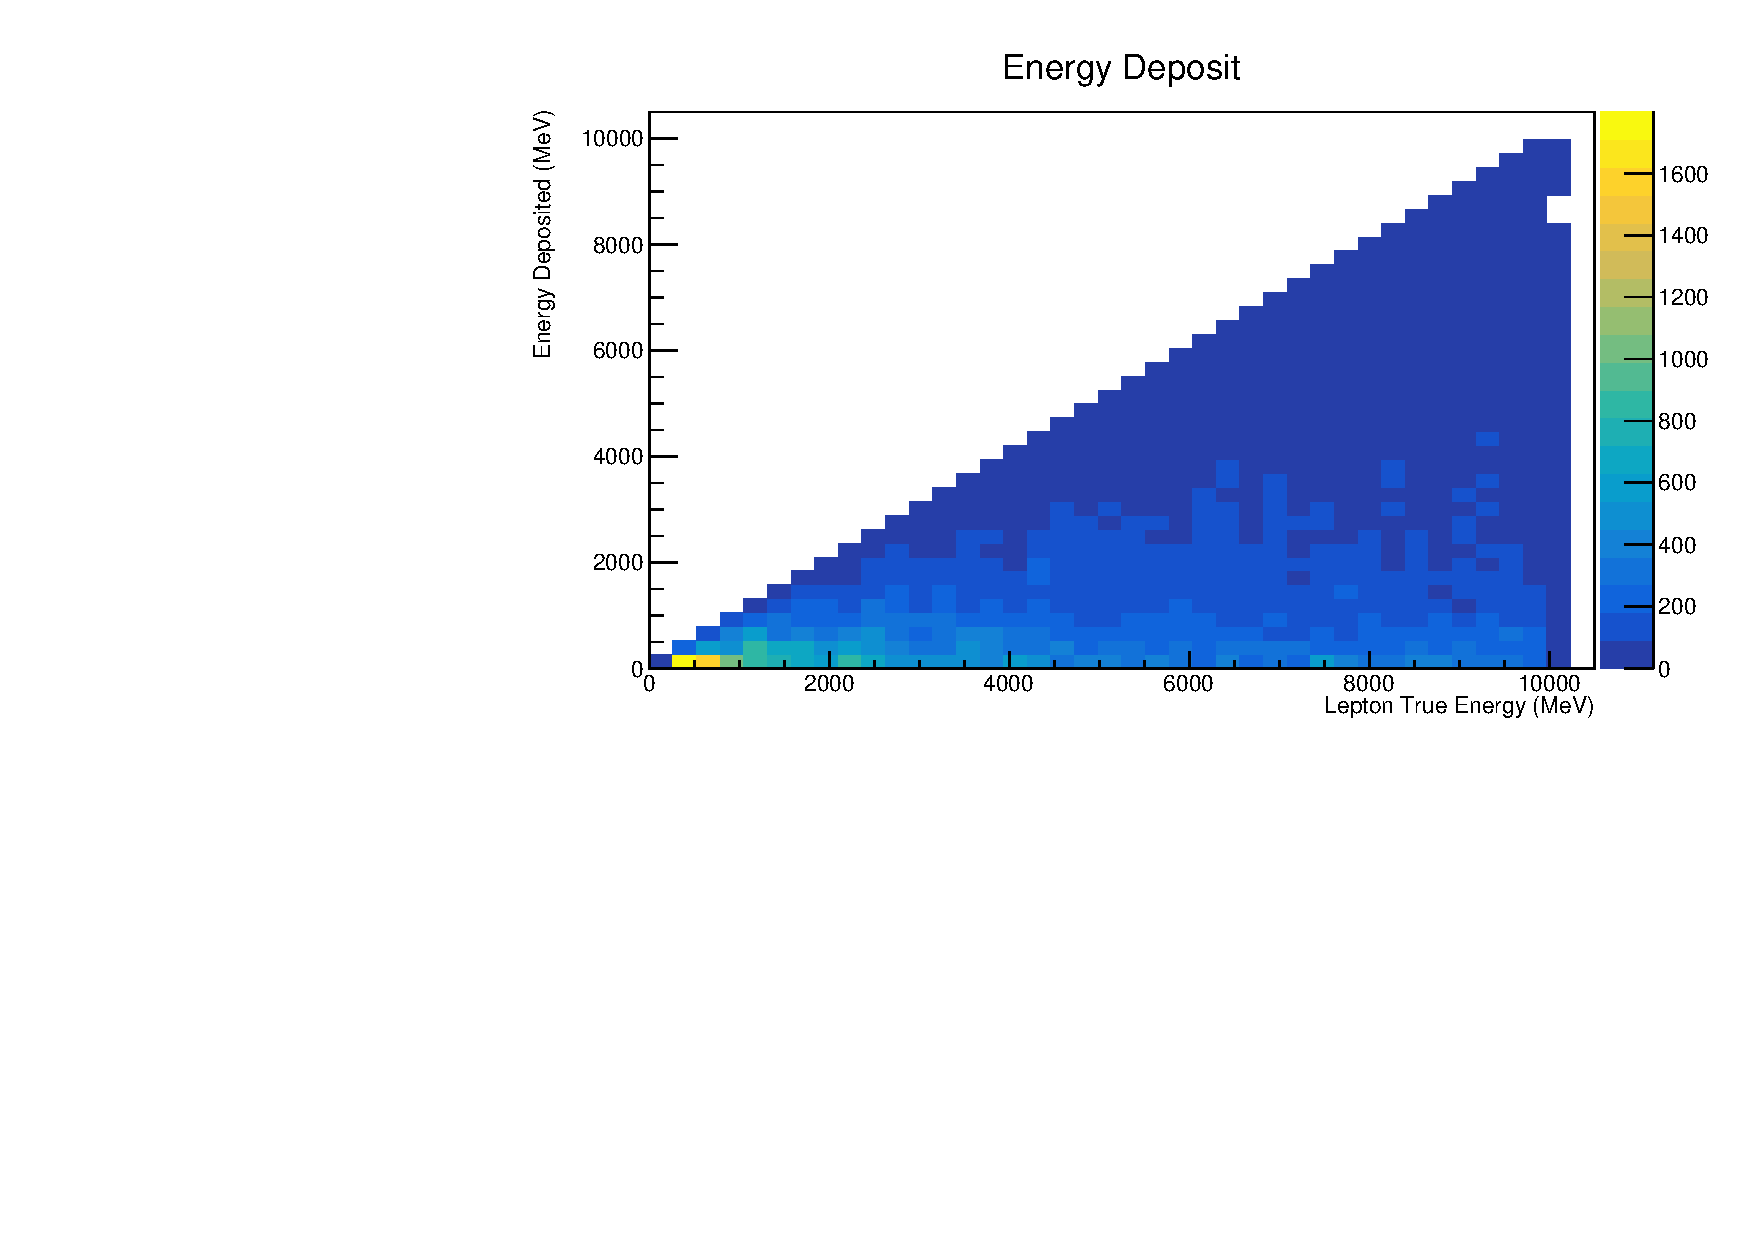
\includegraphics[width=\textwidth]{images/electron_nu_energy_deposit.pdf}
  \caption{}
\end{subfigure}%
\begin{subfigure}{.5\textwidth}
  \centering
  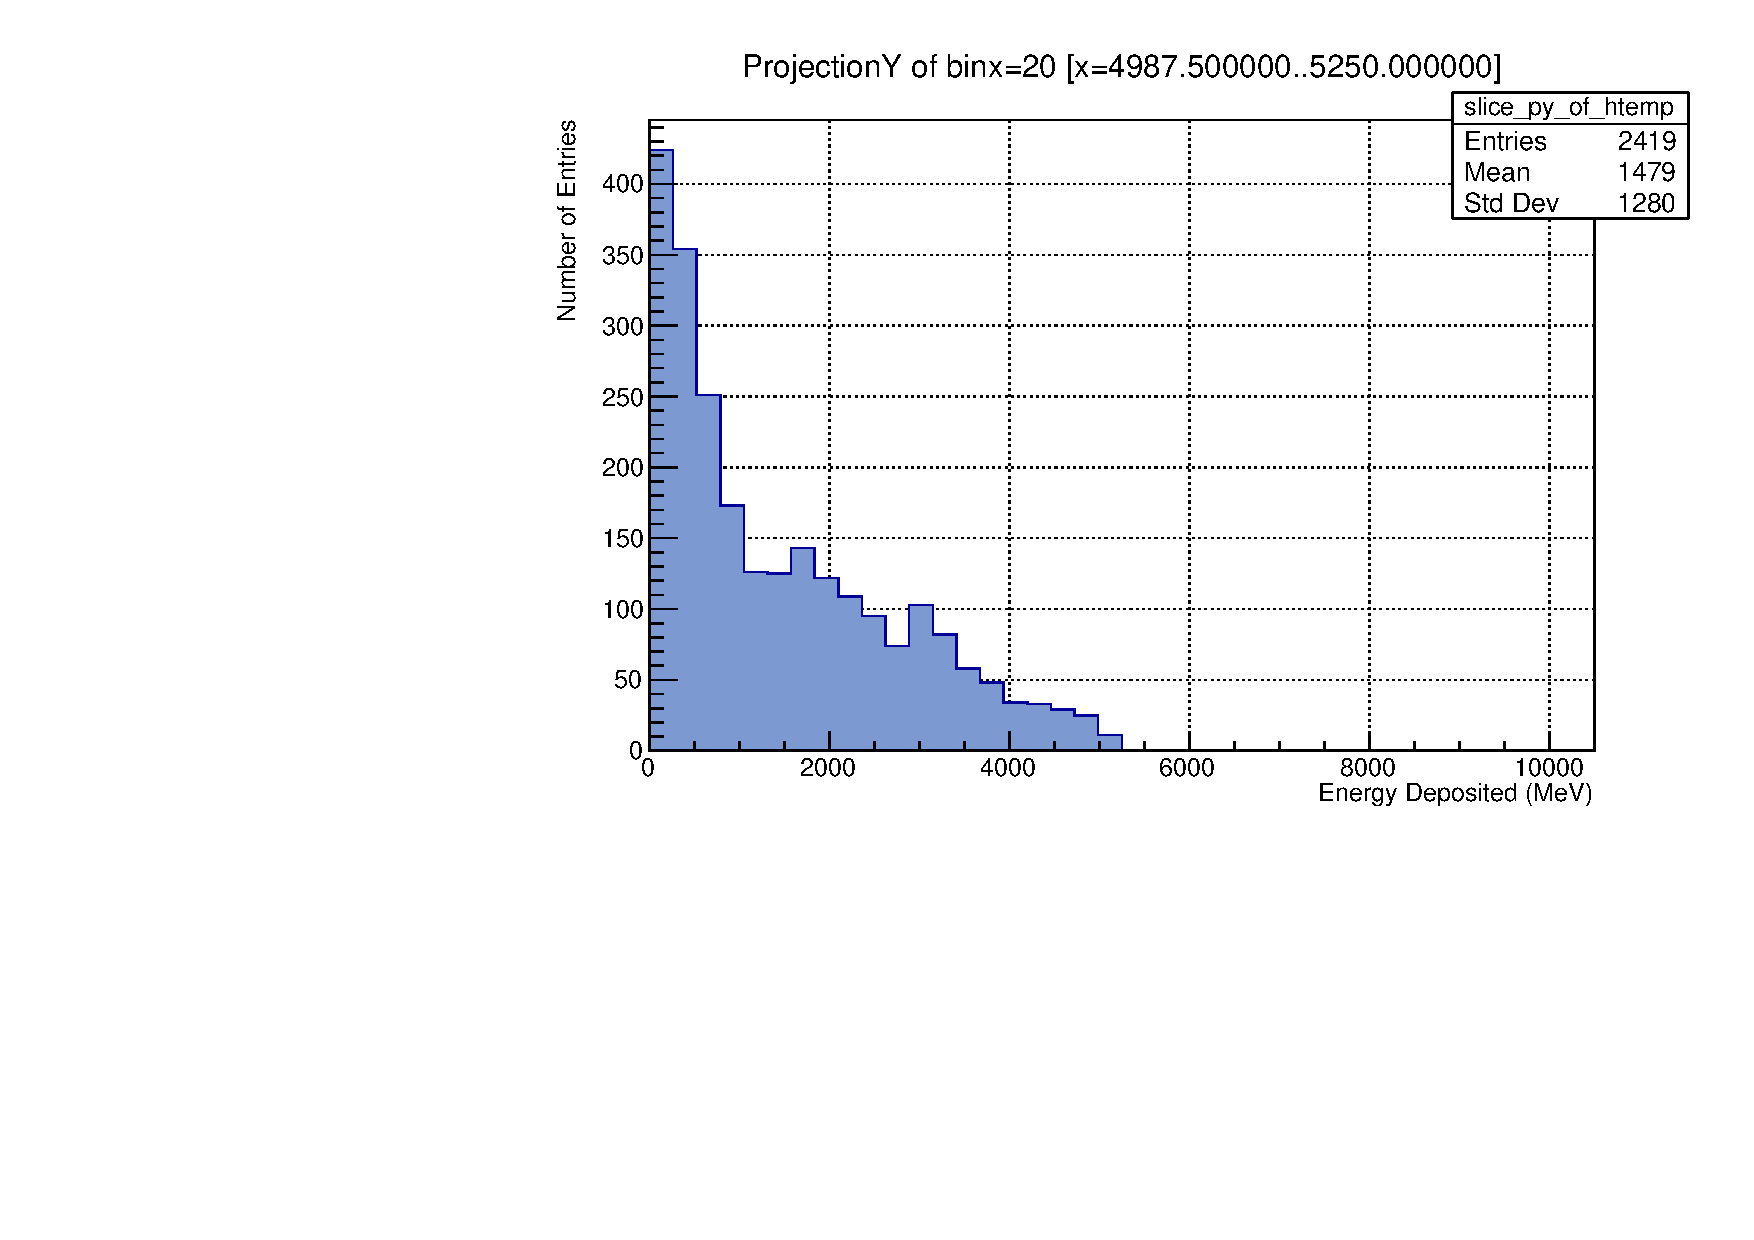
\includegraphics[width=\textwidth]{images/electron_nu_energy_deposit_slice.pdf}
  \caption{}
\end{subfigure}
\caption{Plot-(A) shows a comparison of the energy deposited into the LAr as a function of the input neutrino, which in this case is $\nu_{e}$.
Plot-(B) shows a projection against the y-axis for a single bin.
The maximum allowed total energy deposited is limited to the total energy of the input neutrino.
However, the lower bound for all energies is still, obviously, zero.
Therefore, as the input neutrino energy increases the upper bound also increases.
The mean value of Plot-(B) indicates that even for a maximum allowed total energy of 5~\unit{GeV} the mean (average) energy deposited per event is 1479~\unit{MeV}.
Most interactions deposit less than 2~\unit{GeV} into the LAr, as shown in Figure~\ref{fig:example_energy_deposit}.
}
\label{fig:example_energy_deposit}
\end{figure}

\begin{figure}[]
\centering
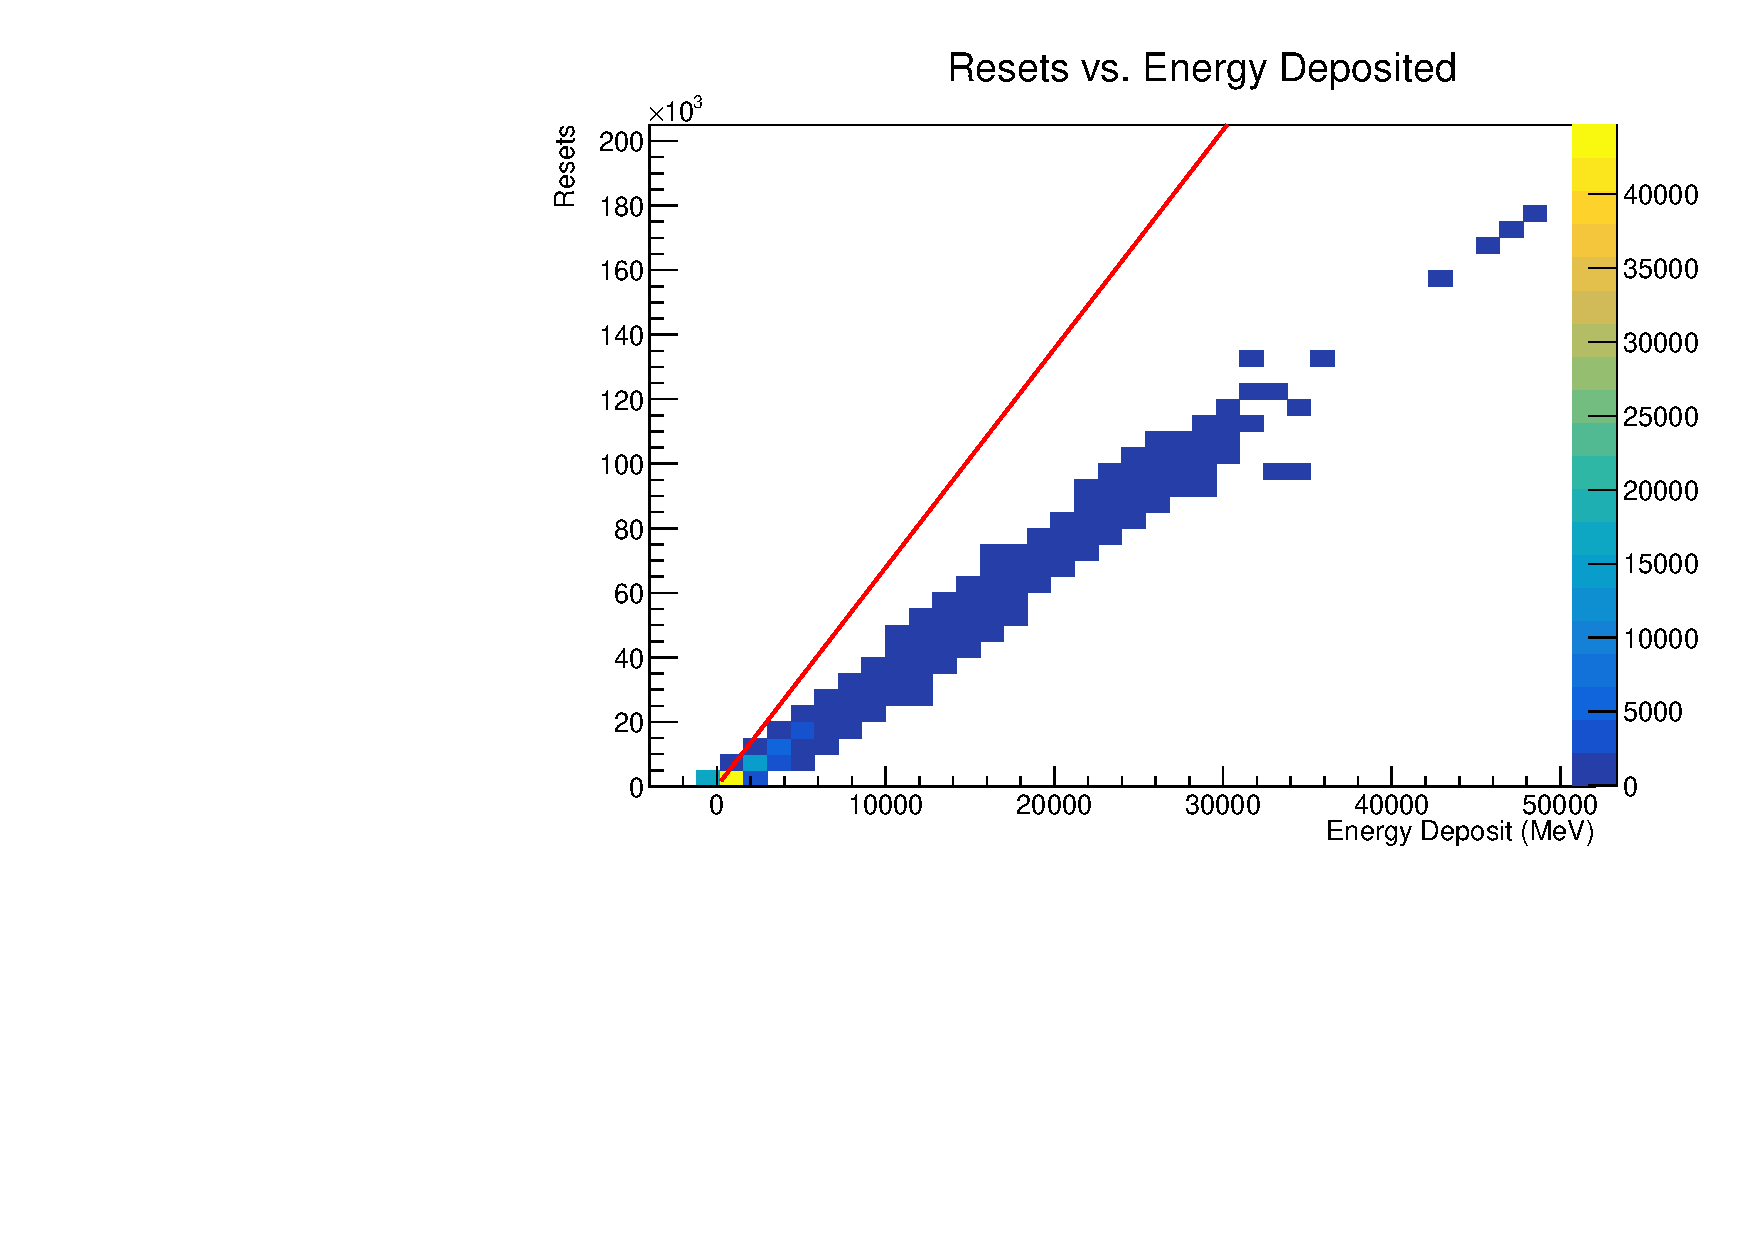
\includegraphics[width=\textwidth]{images/resets_vs_energy_deposit.pdf}
\caption{A relationship between the total number of resets detected in the APA and the energy deposited for $\nu_{e}$ interactions is shown.
The solid red line indicates the maximum number of resets that could be measured for a given energy.
The small distribution of energies below zero correspond to events that produced no resets.
The energy deposited goes above the the threshold limit of 10~\unit{GeV}.
These events carry extra energy from additional leptons which are from pile-up at the DUNE-ND from the FNAL beam.
These data are not included in the energy deposited analysis, or in the integrals as shown in Figure~\ref{fig:compare_integral}.
These high energy deposit events are also not included in the FIFO depth analysis, since these events are beyond the energy range for oscillation measurements.
These events are also removed from Figure~\ref{fig:example_energy_deposit}.
}
\end{figure}~\label{fig:energy_deposit_vs_resets}


%% comparing integral results here
\begin{figure}
\centering
\begin{subfigure}{.5\textwidth}
  \centering
  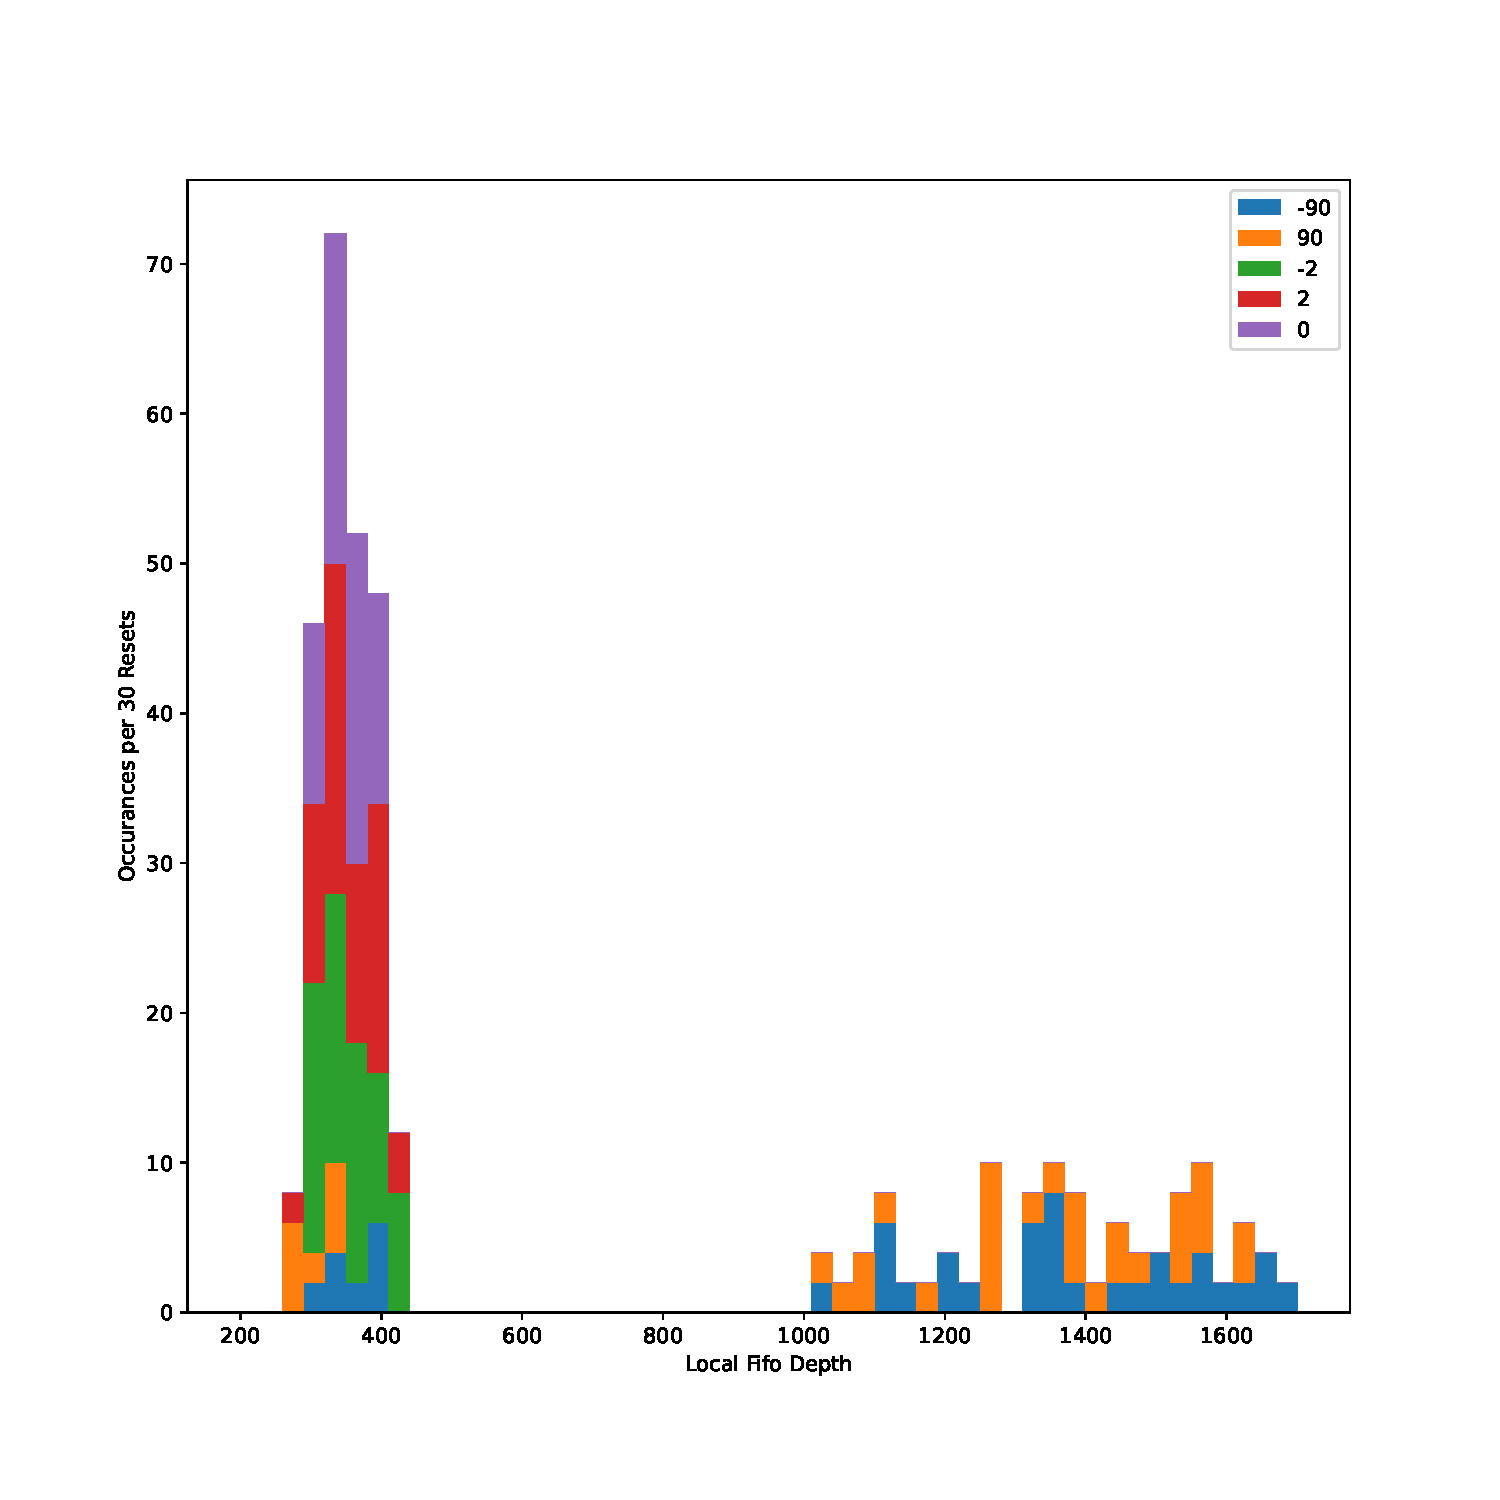
\includegraphics[width=\textwidth]{images/df_theta_cut.pdf}
  \caption{Colored by $\theta_{z}$ direction.}
\end{subfigure}%
\begin{subfigure}{.5\textwidth}
  \centering
  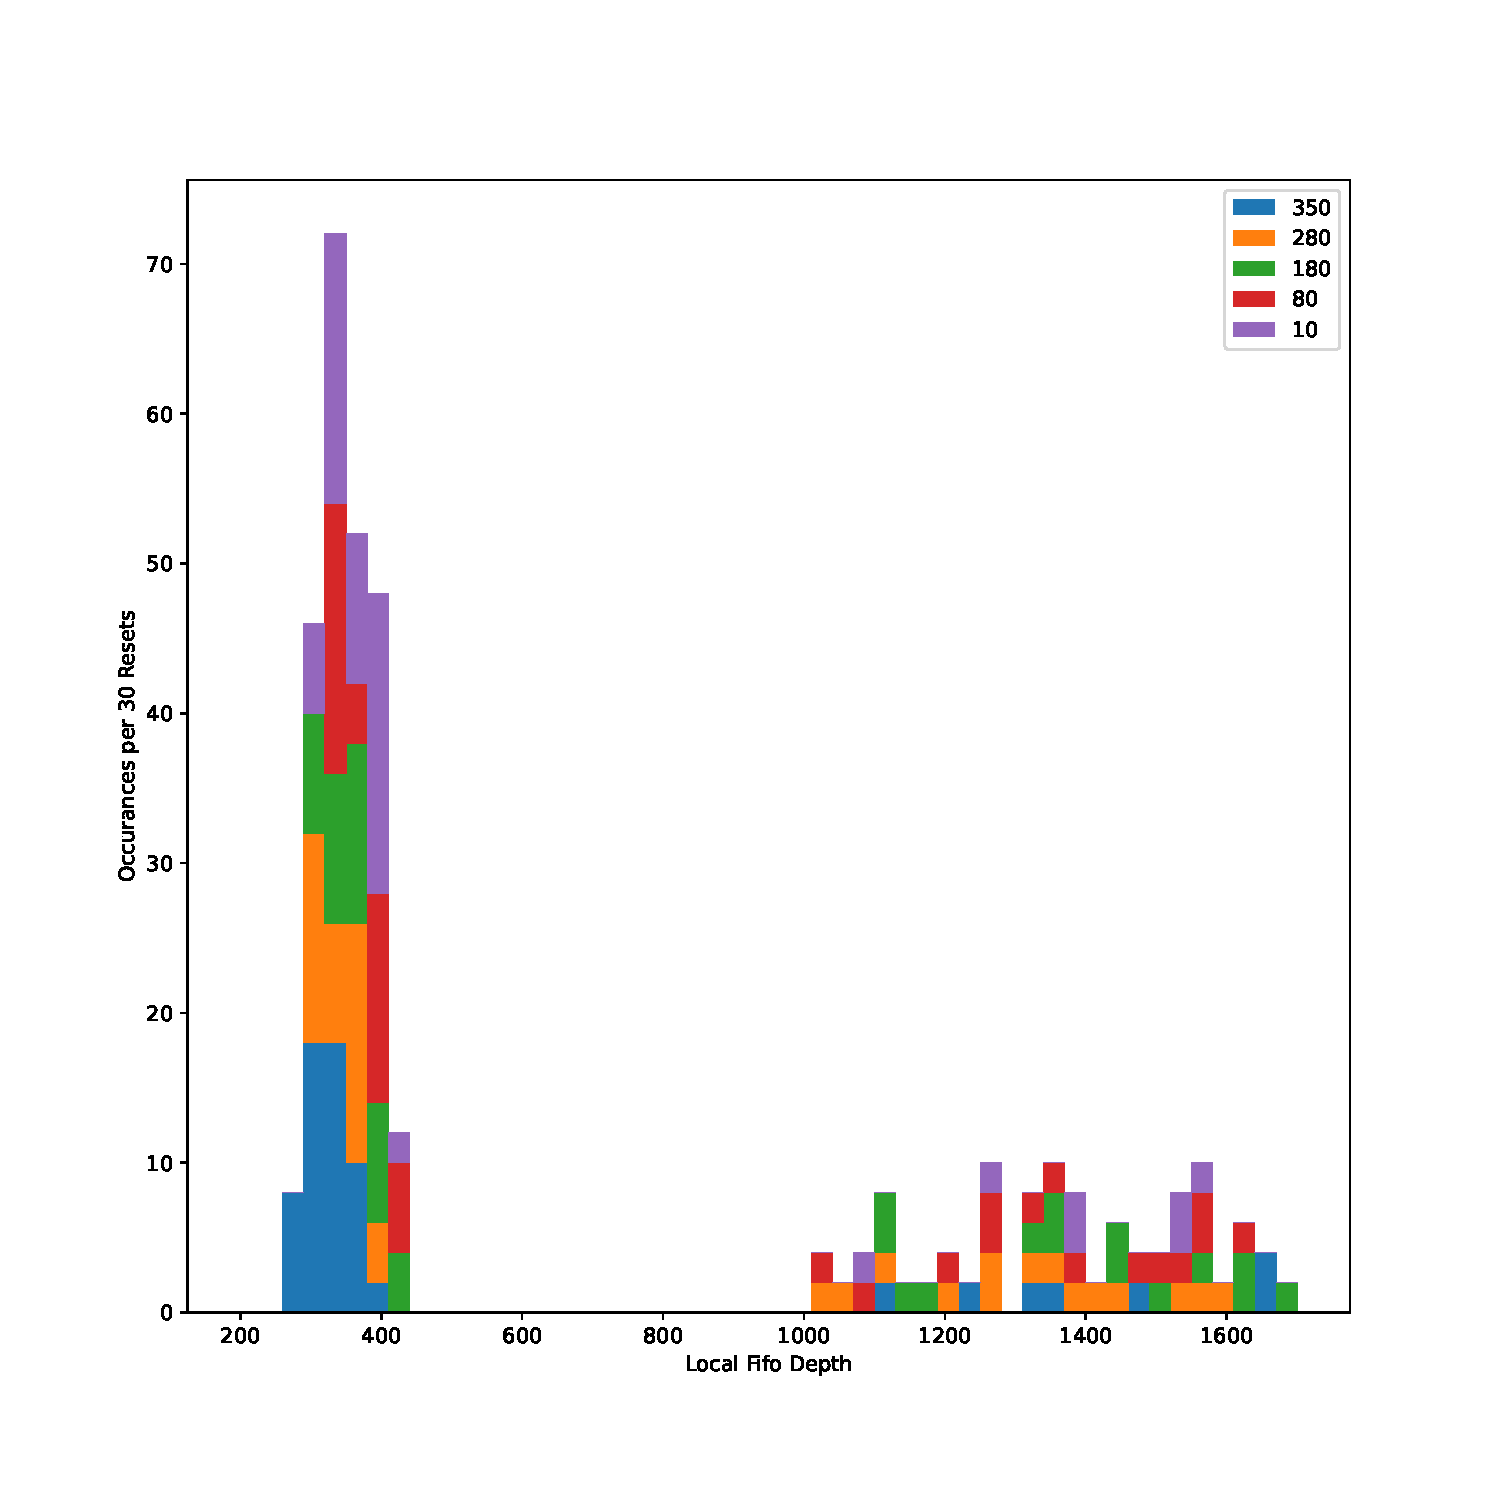
\includegraphics[width=\textwidth]{images/df_zpos_cut.pdf}
  \caption{Colored by Z-position}
\end{subfigure}
\caption{Comparison of Buffer depths as a function of energy for different parameters of $\theta_{z}$ and z-position.
The most important result is shown in Plot-(A), which clearly indicates that only two different parameters account for the distribution of larger local FIFO depths.
As expected, $\theta_{z}$ affects the localization of charge over individual ASICs which affect the local FIFO depth.
Plot-(B) shows the distribution of resets indicated by different z-positions.
Plot-(B) differs in that the second distribution of resets contains elements from each of the different z-positions.
}
\label{fig:compare_integral_zpos_theta}
\end{figure}

\begin{figure}
\centering
\begin{subfigure}{.5\textwidth}
  \centering
  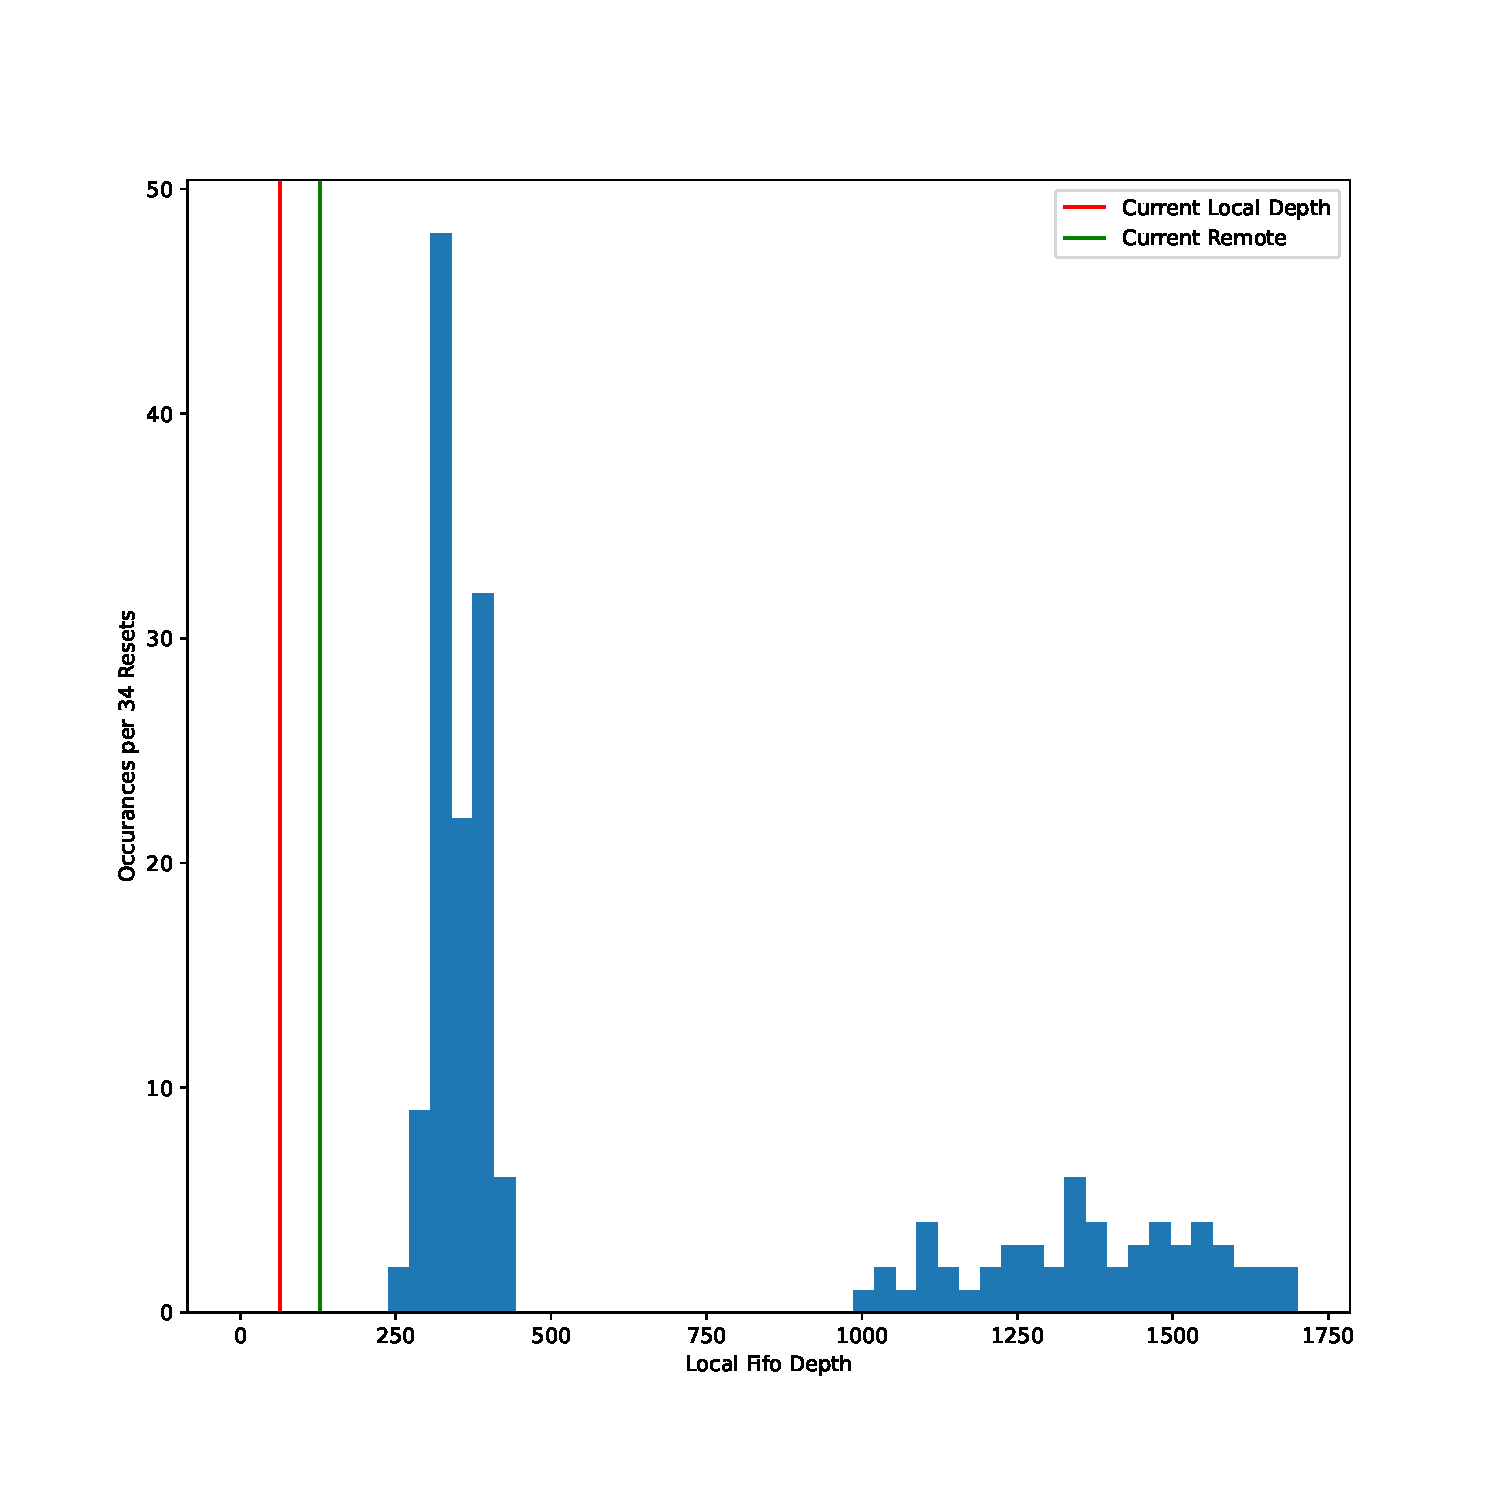
\includegraphics[width=\textwidth]{images/df_nolabel_line.pdf}
  \caption{Comparison of all integrals to current prototype depths.}
\end{subfigure}%
\begin{subfigure}{.5\textwidth}
  \centering
  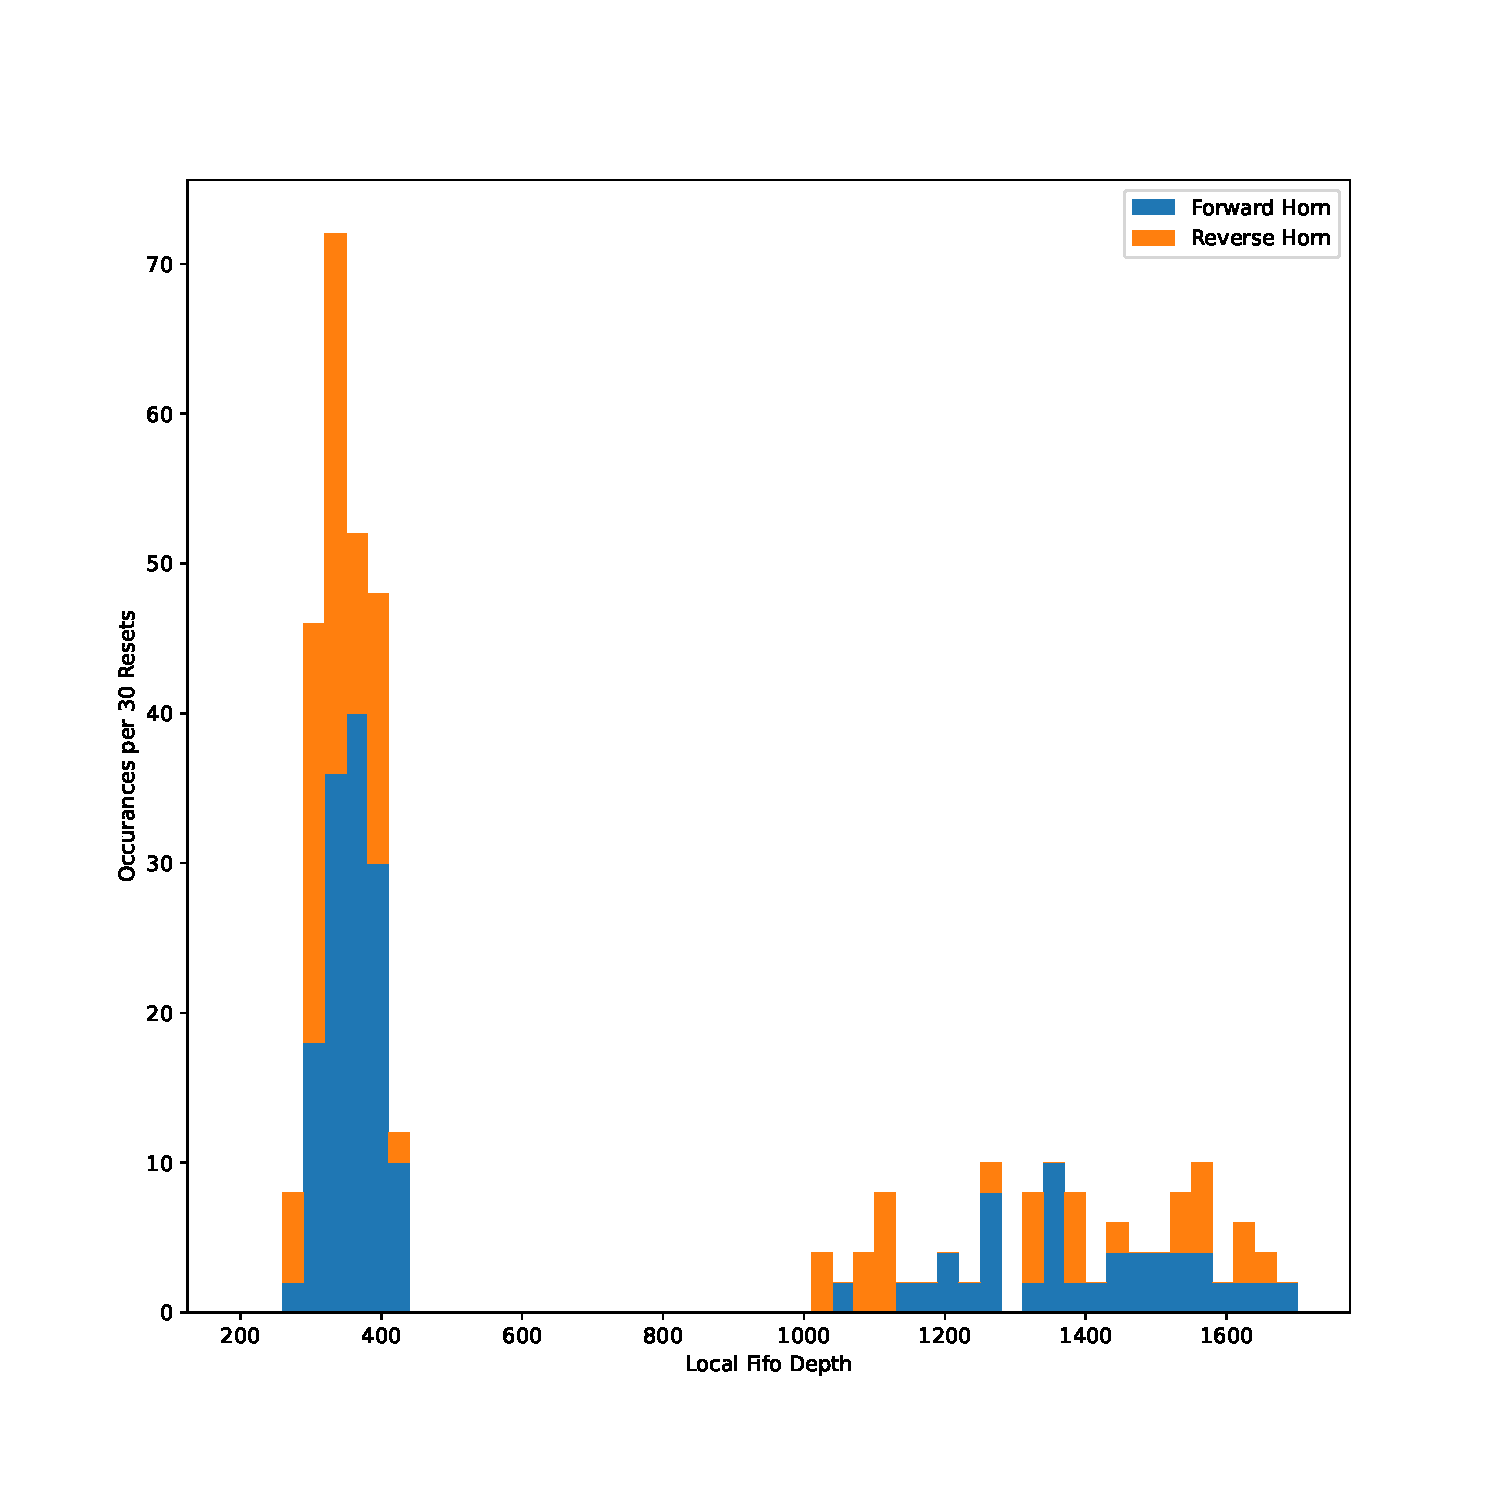
\includegraphics[width=\textwidth]{images/df_horn_cut.pdf}
  \caption{Colored by Z-position}
\end{subfigure}
\caption{Comparison of Buffer depths as in incoming prototype and horn current direction from neutrino beam.}
\label{fig:compare_integral_nolabel}
\end{figure}
